\documentclass[UTF8,a4paper,12pt]{ctexbook} 

\usepackage{graphicx}%学习插入图
\usepackage{verbatim}%学习注释多行
\usepackage{booktabs}%表格
\usepackage{geometry}%图片
\usepackage{amsmath}
\usepackage{amssymb}
\usepackage{listings}%代码
\usepackage{xcolor}  %颜色
\usepackage{enumitem}%列表格式
\setenumerate[1]{itemsep=0pt,partopsep=0pt,parsep=\parskip,topsep=5pt}
\setitemize[1]{itemsep=0pt,partopsep=0pt,parsep=\parskip,topsep=5pt}
\setdescription{itemsep=0pt,partopsep=0pt,parsep=\parskip,topsep=5pt}
\usepackage{tcolorbox}
\usepackage{algorithm}  %format of the algorithm
\usepackage{algorithmic}%format of the algorithm
\usepackage{multirow}   %multirow for format of table
\usepackage{tabularx} 	%表格排版格式控制
\usepackage{array}	%表格排版格式控制
\usepackage{hyperref} %超链接 \url{URL}
\usepackage{tikz}
\usepackage{dirtree}


\usetikzlibrary{intersections,
	positioning,
	petri,
	backgrounds,
	fit,
	decorations.pathmorphing,
	arrows,
	arrows.meta,
	bending,
	calc,
	intersections,
	through,
	backgrounds,
	shapes.geometric,
	quotes,
	matrix,
	trees,
	shapes.symbols,
	graphs,
	math,
	patterns,
	external}
\CTEXsetup[format+={\flushleft}]{section}

%%%% 设置图片目录
\graphicspath{{figure/}}

%%%% 段落首行缩进两个字 %%%%
\makeatletter
\let\@afterindentfalse\@afterindenttrue
\@afterindenttrue
\makeatother
\setlength{\parindent}{2em}  %中文缩进两个汉字位

%%%% 下面的命令重定义页面边距,使其符合中文刊物习惯 %%%%
\addtolength{\topmargin}{-54pt}
\setlength{\oddsidemargin}{0.63cm}  % 3.17cm - 1 inch
\setlength{\evensidemargin}{\oddsidemargin}
\setlength{\textwidth}{14.66cm}
\setlength{\textheight}{24.00cm}    % 24.62

%%%% 下面的命令设置行间距与段落间距 %%%%
\linespread{1.4}
\setlength{\parskip}{0.5\baselineskip}
\geometry{left=1.6cm,right=1.8cm,top=2cm,bottom=1.7cm} %设置文章宽度
\pagestyle{plain} 		  %设置页面布局

%代码效果定义
\definecolor{mygreen}{rgb}{0,0.6,0}
\definecolor{mygray}{rgb}{0.5,0.5,0.5}
\definecolor{mymauve}{rgb}{0.58,0,0.82}
\lstset{ %
	backgroundcolor=\color{white},   % choose the background color
	basicstyle=\footnotesize\ttfamily,      % size of fonts used for the code
	%stringstyle=\color{codepurple},
	%basicstyle=\footnotesize,
	%breakatwhitespace=false,         
	%breaklines=true,                 
	%captionpos=b,                    
	%keepspaces=true,                 
	%numbers=left,                    
	%numbersep=5pt,                  
	%showspaces=false,                
	%showstringspaces=false,
	%showtabs=false,        
	columns=fullflexible,
	breaklines=true,                 % automatic line breaking only at whitespace
	captionpos=b,                    % sets the caption-position to bottom
	tabsize=4,
	commentstyle=\color{mygreen},    % comment style
	escapeinside={\%*}{*)},          % if you want to add LaTeX within your code
	keywordstyle=\color{blue},       % keyword style
	stringstyle=\color{mymauve}\ttfamily,     % string literal style
	frame=L,
	xleftmargin = .079\textwidth,
	rulesepcolor=\color{red!20!green!20!blue!20},
	% identifierstyle=\color{red},
	language=c++,
}
 \author{\kaishu 郑华}
 \title{\heiti U3D笔记}
 
\begin{document}          %正文排版开始
 	\maketitle
 	\tableofcontents

\chapter{基础}
	入门参考:\url{https://unity3d.com/cn/learn/tutorials}
	
	\section{如何将脚本与具体对象绑定}
		\begin{enumerate}
			\item 右键\verb|asset|文件夹,创建C\#脚本
			\item 编写脚本
			\item 将\verb|asset |中的脚本拖拽到 \verb|hiearch |视图中的\verb|MainCamera |中
			\item 如果脚本是作用于场景中的某个物体,\textbf{则将该脚本拖拽到该物体上}
		\end{enumerate}
	
	\section{序列化-  [SerializedField]}
		\textit{通常情况下},GameObject上挂的MonoBehaviour脚本中的\textbf{私有变量}\textit{不会显示在Inspector面板上},即不会被序列化。
		
		\textbf{但如果指定了SerializedFiled特性},就可以被序列化了。
		
		\begin{lstlisting}
	public class Test : MonoBehaviour 
	{
		public string Name;
		[SerializeField]
		private int Hp; 
	}
		\end{lstlisting}
		
		\begin{figure}[H]
			\centering
			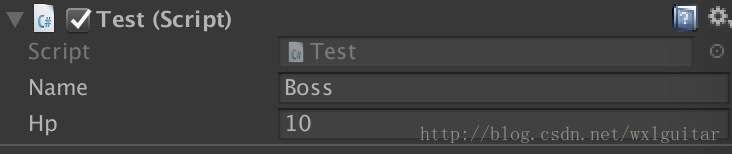
\includegraphics[scale=0.8]{SerilizedFiled.jpg}
			\caption{序列化操作 -在Inspector上显示}
		\end{figure}
	
	\section{常用技巧}
		\begin{itemize}
			\item \verb|ctrl + d| 复制
			\item \verb|shift + 鼠标 | 等比例缩放 
			\item \verb|shift + alt + 鼠标 | 原地等比例缩放
			\item \verb|在Unity 编辑器中输入汉字 | 需要借助其他文本拷贝粘贴
			\item \verb|q、w、e、r、t |在操作UI时尽量使用 T,以避免z轴发生的变化 
		\end{itemize}
	
	\section{MonoBehaviour 生命周期、渲染管线}
		
		\subsection{脚本渲染流程}
			\begin{figure}[H]
				\centering
				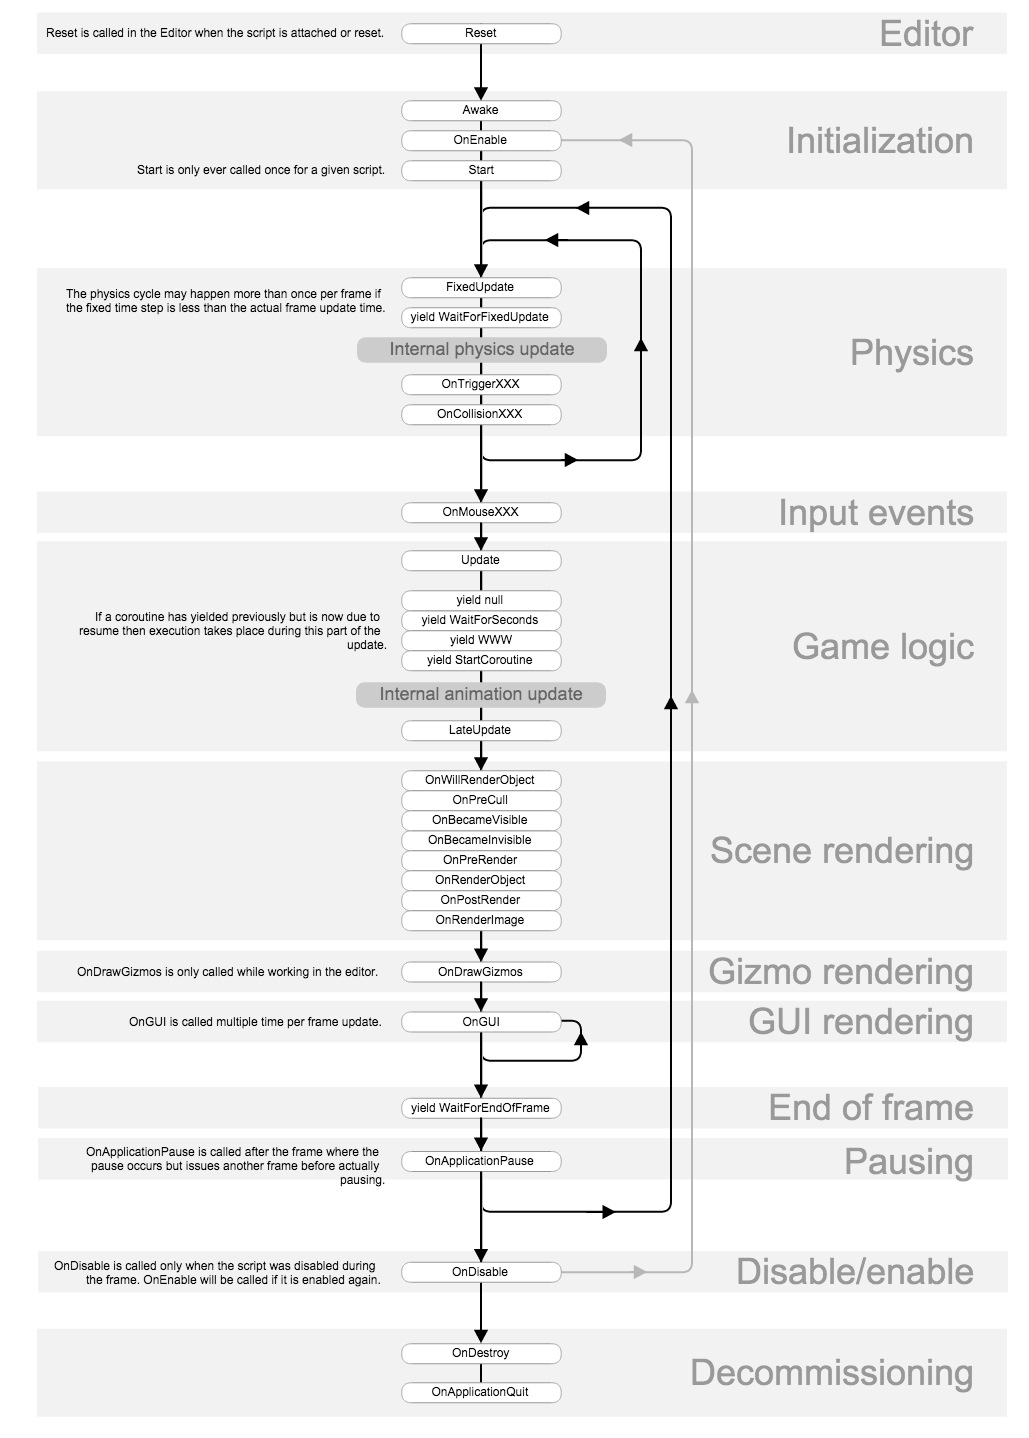
\includegraphics[scale=0.44]{scriptLifeCircle.jpg}
				\caption{脚本生命周期核心方法}
			\end{figure}
			
			\clearpage
			\begin{figure}[H]
				\centering
				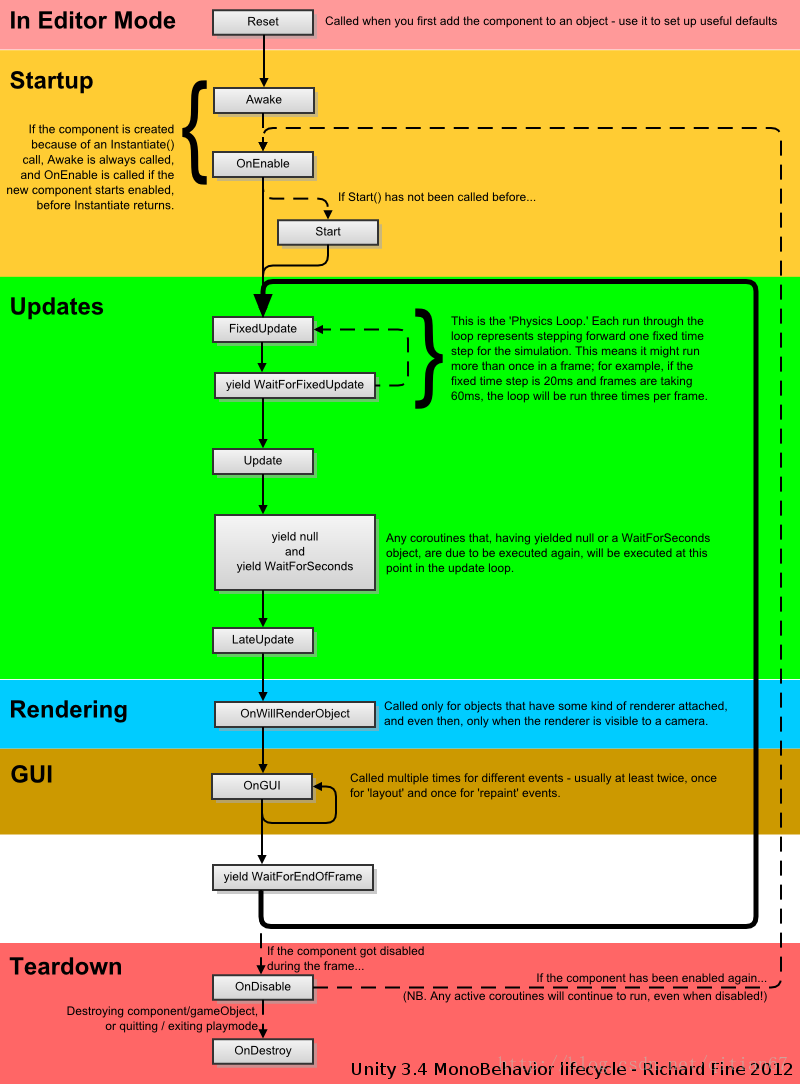
\includegraphics[scale=0.78]{LifeCicle.png}
				\caption{简要核心方法}
			\end{figure}
		
		update:当其\textbf{所在的物体}属于未激活的话(\verb|active为false|),\textit{该物体上所有脚本中包含的协程代码都是不会被执行的}。
		\subsection{核心方法}
			\begin{enumerate}
				\item \verb|Reset |:
				\item \verb|Awake |:脚本唤醒函数,\textbf{当游戏对象被创建的时候},\textit{游戏对象}\textbf{绑定的脚本会在该帧(Frame)内}\textit{执行Awake() 函数},\textbf{无论}脚本是否处于激活(\textbf{enable})状态。
				\item \verb|OnEnable |:激活函数,当脚本被激活时调用。
				\item \verb|Start |:该函数在脚本被激活的时候执行,位于Awake之后,该函数同样也是在游戏对象被创建的帧里,\textbf{不同的是},如果脚本处于不激活状态(\verb|MonoBehaviour.enable = false|), start 函数是不会执行的。
				\item \verb|FixedUpdate |:
				\item \verb|yield WaitForFixedUpdate |:
				\item \verb|OnTriggerXXX |:
				\item \verb|Update |:\textbf{只要处于激活状态的脚本},\textit{都会在每一帧里调用Update() 函数},该函数也是最为常用的一个函数,用来更新逻辑。
				\item \verb|LateUpdate |:延迟更新函数
				\item \verb|OnWillRenderObject |:
				\item \verb|OnGUI |:绘制界面函数。 
				\item \verb|yield WaitForEndOfFrame |:
				\item \verb|OnDisable |:
				\item \verb|OnDestroy |:在当前脚本销毁时调用该函数。
			\end{enumerate}
		
	\section{Unity 委托}
		
		\paragraph{定义}\verb|public delegate void MyDelegate(int num);|
		
			\textbf{委托}就是\verb|C#|封装的\textbf{C++的函数指针}。
			
			定义一个委托MyDelegate,如同定义一个类一样,此时的委托没有经过实例化是无法使用的,而他的实例化必须接收一个返回值和参数都与他等同的函数,此处的委托MyDelegate只能接收返回值为void,参数为一个int的函数
			
		\paragraph{实例化委托}:\verb|MyDelegate _MyDelegate=new MyDelegate(TestMod);|
			
			以\verb|TestMod|函数实例化一个\verb|MyDelegate|类型的委托\verb|_MyDelegate|,此处\verb|TestMod|函数的定义就应如下:
				
			\verb|public void TestMod(int _num);|
				
			之后调用\verb|_MyDelegate(100)|时就完全等同于调用\verb|TestMod(100)|
		
		
		
	\section{Unity 协程}
		\subsection{开启方式}
			协程:协同程序,在主程序运行的同时,开启另外一段逻辑处理,来协同当前程序的执行。
			
			\paragraph{StartCoroutine(string MethodName)}
				\begin{itemize}
					\item 参数是方法名					
					\item 形参方法可以有返回值
				\end{itemize}
			
			\paragraph{StartCoroutine(IEnumerator method)}
				\begin{itemize}
					\item 参数是方法名(\verb|TestMethod()|),方法中\textbf{可以包含多个参数}
					\item \verb|IEnumrator| 类型的方法不能含有\verb|ref或者out| 类型的参数,\textbf{但可以含有被传递的引用}
					\item \textbf{必须有有返回值},且返回值类型为\verb|IEnumrator|,返回值使用(\textit{yield retuen +表达式或者值},或者 \textit{yield break})语句	
			\end{itemize}
		
		\subsection{终止方式}
			\paragraph{StopCoroutine(string MethodName)}
				只能终止指定的协程
			
			\paragraph{StopAllCoroutine()}
				终止所有协程
				
		\subsection{yield 方式}
			\paragraph{yield return}
				挂起,\textbf{程序遇到}\verb|yield|\textbf{关键字时会被挂起},暂停执行,\textbf{等待条件满足时从当前位置继续执行}
				
				\begin{itemize}
					\item \verb|yield return 0| or \verb|yield return null|:程序在下一帧中从当前位置继续执行
					\item \verb|yield return 1,2,3,......|: 程序等待1,2,3...帧之后从当前位置继续执行
					\item \verb|yield return new WaitForSeconds(n)|:程序等待n秒后从当前位置继续执行
					\item \verb|yield new WaitForEndOfFrame()|:在所有的渲染以及GUI程序执行完成后从当前位置继续执行
					\item \verb|yield new WaitForFixedUpdate()|:所有脚本中的FixedUpdate()函数都被执行后从当前位置继续执行
					\item \verb|yield return WWW()|:等待一个网络请求完成后从当前位置继续执行
					\item \verb|yield return StartCoroutine()|:等待一个协程执行完成后从当前位置继续执行
				\end{itemize}
			
			\paragraph{yield break}
				如果使用\verb|yield break|语句,将会导致\textbf{如果协程的执行条件不被满足},\textit{不会从当前的位置继续执行程序,而是直接从当前位置跳出函数体,回到函数的根部}
				
				\color{blue}相当于:\textbf{return; + 暂停}\color{black}
				
		\subsection{执行原理}
			协程函数的返回值是\verb|IEnumerator|,它是一个迭代器,\textbf{可以把它当成执行一个序列的某个节点的指针},它提供了两个重要的接口,分别是\verb|Current|(返回当前指向的元素)和\verb|MoveNext()|(将指针向后移动一个单位,\textit{如果移动成功,则返回true})
			
			\verb|yield|关键词\textbf{用来声明序列中的下一个值或者是一个无意义的值},如果使用\verb|yield return x|(x是指一个具体的对象或者数值)的话,那么\verb|MoveNext|返回为\verb|true|并且\verb|Current|被赋值为\verb|x|,如果使用\verb|yield break|使得\verb|MoveNext()|返回为\verb|false|
			
			如果\verb|MoveNext|函数返回为\verb|true|\textbf{意味着协程的执行条件被满足,则能够从当前的位置继续往下执行}。否则不能从当前位置继续往下执行。	

	\paragraph{委托+协程}
		\url{https://blog.csdn.net/qq992817263/article/details/51514449}
		
		\begin{itemize}
			\item 实现延时
			\item 实现给定函数传参
			\item 实现特定功能
		\end{itemize}
	
		\begin{lstlisting}
	// 延时执行

	// <param name="action">执行的委托</param>
	// <param name="obj">委托的参数</param>
	// <param name="delaySeconds">延时等待的秒数</param>
	public IEnumerator DelayToInvokeDo(Action<GameObject> action, GameObject obj,float delaySeconds)
	{
		yield return new WaitForSeconds(delaySeconds); // delaySeconds 后执行
		action(obj); // 特定功能
	}
	// 使用例子
	StartCoroutine(
		DelayToInvokeDo(
			delegate(GameObject task) {
				task.SetActive(true);
				task.transform.position = Vector3.zero;
				task.transform.rotation = Quaternion.Euler(Vector3.zero);
				task.doSomethings();
			},
			/*传参*/GameObject.Find("task1"),
			1.5f)/*End 匿名委托*/
		);/*End 协程初始*/
		\end{lstlisting}
		
\chapter{事件}
	\section{必然事件}
		继承自\verb|MonoBehaviour 类|后,自动会\textbf{按序}\textit{提供以下方法}:
		
		\begin{itemize}
			\item \verb|Awake()|:在加载场景时运行,用于在游戏开始前完成变量初始化、以及游戏状态之类的变量。
			\item \verb|Start()|:在第一次启动游戏时执行,用于游戏对象的初始化,在\verb|Awake() |函数之后。
			\item \verb|Update()|:是在每一帧运行时必须执行的函数,用于更新场景和状态。
			\item \verb|FixedUpdate()|:与\verb|Update() |函数相似,但是在固定的物理时间后间隔调用,用于物理状态的更新。
			\item \verb|LateUpdate()|:是在\verb|Update() |函数执行完成后再次被执行的,有点类似收尾的东西。 
		\end{itemize}
			
	\section{碰撞事件}
		U3D 的碰撞检测。具体分为三个部分进行实现,碰撞发生进入时、碰撞发生时和碰撞结束,理论上不能穿透
		
		\begin{itemize}
			\item \verb|OnCollisionEnter(Collision collision)| 当碰撞物体间刚接触时调用此方法
			\item \verb|OnCollisionStay(Collision collision)| 当发生碰撞并保持接触时调用此方法
			\item \verb|OnCollisionExit(Collision collision)| 当不再有碰撞时,既从有到无时调用此函数
		\end{itemize}

	\section{触发器事件}
		类似于 红外线开关门, 有个具体的范围,然后进入该范围时,执行某种动作,离开该范围时执行某种动作。类似于物体于一个透明的物体进行碰撞检测,理论上需要穿透,在U3D 中通过勾选 \verb|Is Trigger| 来确定该物体是可以穿透的。
		
		\begin{itemize}
			\item \verb|OnTriggerEnter() | 当其他碰撞体进入触发器时,执行该方法
			\item \verb|OnTriggerStay() | 当其他碰撞体停留在该触发器中,执行该方法
			\item \verb|OnTriggerExit() | 当碰撞体离开该触发器时,调用该方法
		\end{itemize}
		

\chapter{实体-人物、物体、组件}
		
	\section{实体类} \verb|GameObject 类|,游戏基础对象,用于填充世界。
		\paragraph{复制}
			\verb|Instantiate(GameObject)| 或 \verb|Instantiate(GameObject, position, rotation)|
			
			\begin{itemize}
				\item \verb|GameObject |指生成克隆的\textbf{游戏对象},也可以是\textbf{Prefab 的预制品}
				\item \verb|position |克隆对象的初始位置,类型为\verb|Vector3|
				\item \verb|rotation |克隆对象的初始角度,类型为\verb|Quaternion|
			\end{itemize} 
		
		\paragraph{销毁}
			\verb|Destroy(GameObject xx)- 立即销毁 |或 \verb|Destroy(GameObject xx, Time time)- 几秒后销毁|
			
		\paragraph{可见否}
			通过设置该参数调整该实体是否可以在游戏中显示,具体设置方法为\verb|gameObject.SetActive(true) 为可以显示,false 则隐藏|
		
		\paragraph{游戏中获取}
			\begin{enumerate}
				\item 在整个场景中寻找名为xx的游戏对象,并赋予obj 变量
					
					\verb|obj = GameObject.Find("xx");|
					
				\item 当需要获取某个\verb|gameObject| 下的组件时,使用\verb|Transform.Find.GetComponent|
					
					\verb|gameObjVar1.transform.Find("ImageItemIcon/TextMonthCardLeftDays").\label{GetComponen\left( }t<Text>().text = "xx";|
				
				\item 但是设置为激活状态则需要如下通过\verb|gameObject|进行设置。
				
					\verb|obj = gameObjVar1.transform.Find("xx/xx").gameObject.SetActive(true);|
			\end{enumerate}
	\section{Prefabs -预设体}
		prefabs基础:\url{https://www.cnblogs.com/yuyaonorthroad/p/6107320.html}
		
		动态加载Prefabs:\url{https://blog.csdn.net/linshuhe1/article/details/51355198}
		
		在进行一些功能开发的时候,我们常常将一些\textbf{能够复用的对象}制作成.\textbf{prefab的预设物体},然后将预设体存放到Resources目录之下,使用时再动态加载到场景中并进行实例化。例如:子弹、特效甚至音频等,都能制作成预设体。
		
		\subparagraph{概念} 组件的集合体, 预制物体可以实例化成游戏对象.
		\subparagraph{作用} 可以重复的创建具有相同结构的游戏对象。	
		
		\subsection{预设动态加载到场景}
			\paragraph{预设体资源加载}\verb|->|
			
				假设预设体的位置为下图所示
				\begin{figure}[H]
					\centering
					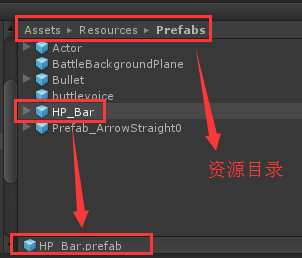
\includegraphics[scale=0.6]{Prefab-1.png}
					\caption{Prefab 资源位置}
				\end{figure}
			
				\begin{lstlisting}[xleftmargin = .079\textwidth, frame = L]
	//加载预设体资源
	GameObject hp_bar = (GameObject)Resources.Load("Prefabs/HP_Bar");				
				\end{lstlisting}
				
			通过上述操作,实现从资源目录下\textbf{载入}\verb|HP_Bar.prefab|\textbf{预设体},\textbf{用}一个\verb|GameObject|\textbf{对象来存放},此时该预设物体并未真正载入到场景中,因为还未进行实例化操作。
			
			\paragraph{预设体实例化}\verb|->|
			
				实例化使用的是\verb|MonoBehaviour.Instantiate|函数来完成的,\textbf{其实质就是从预设体资源中克隆出一个对象},它\textit{具有与预设体完全相同的属性},并且被加载到当前场景中
				
				完成以上代码之后,在当前场景中会出现一个实例化之后的对象,并且其父节点默认为当场的场景最外层,如下图所示。
					\begin{figure}[H]
						\centering
						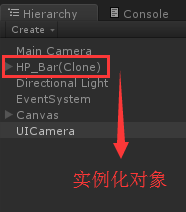
\includegraphics[scale=0.8]{Prefab-2.png}
						\caption{Prefab 实例后位置}
					\end{figure}
				
			\paragraph{实例化对象属性设置}\verb|->|
				
				完成上述步骤之后,我们已经可以在场景中看到实例化之后的对象,但是通常情况下我们\textbf{希望}我们的\textbf{对象之间层次感分明},而且这样也方便我们进行对象统一管理,而不是在Hierarchy中看到一大堆并排散乱对象,所以我们\textbf{需要为对象设置名称以及父节点等属性}。
			
				\verb|-->Notice:|常见错误:对\textbf{未初始化}的\verb|hp_bar|进行属性设置,\textbf{设置之后的属性在实例化之后无法生效}。这是\textit{因为我们最后在场景中}\textbf{显示的其实并非实例化前的资源对象},\textbf{而是一个克隆对象},\color{blue}\textit{所以假如希望设置的属性在最后显示出来的对象中生效,我们需要对实例化之后的对象进行设置}。\color{black}
			
			  正确的设置代码如下,可以看到\textbf{实例化对象}已成功挂在到\textbf{父节点Canvas}上,在层次视图效果如下图所示:
			  	\begin{lstlisting}[xleftmargin = .079\textwidth, frame = L]
	GameObject hp_bar = (GameObject)Resources.Load("Prefabs/HP_Bar");
	
	//搜索画布的方法!
	GameObject mUICanvas = GameObject.Find("Canvas");
	hp_bar = Instantiate(hp_bar);
	hp_bar.transform.parent = mUICanvas.transform;
			  	\end{lstlisting}
			  	
			  	\begin{figure}[H]
			  		\centering
			  		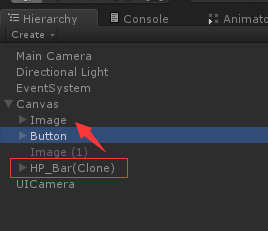
\includegraphics[scale=0.8]{Prefab-3.png}
			  		\caption{Prefab对象 设置父子关系}
			  	\end{figure}
		  	
		  		\subparagraph{简化写法}上述实例步骤与属性设置代码可以简化为
		  			\begin{lstlisting}[xleftmargin = .079\textwidth, frame = L]
	GameObject hp_bar = (GameObject)Instantiate(Resources.Load("Prefabs/HP_Bar"));
	GameObject mUICanvas = GameObject.Find("Canvas");
	hp_bar.transform.parent = mUICanvas.transform;	  				
		  			\end{lstlisting}
		  	
		  	\paragraph{预制体添加脚本}
		  		在预制体上不能直接添加脚本,首先需要将其拖入场景,然后再对其操作,这个时候可以添加脚本,添加组件等,在完成这些操作后,在Inspector 选项中选中 Apply,然后删除其在场景中的刚才拖过来的,即可。		
	\section{获取实体上的组件}
		\paragraph{调用方式}\verb|GameObject.GetComponent<Type>().xx = xx;|
			
			\begin{itemize}
				\item \verb|cube1.GetComponent<RigidBody>().mass = 20;| //设置重量
				\item \verb|cube1.GetComponent<BoxCollider>().isTrigger = true;| //\textbf{开启Trigger 穿透方式}检测
				\item \verb|cube2.GetComponent<Test>().enable = false;| //\textbf{禁用Test脚本}
			\end{itemize}
	
	\section{物理作用实体类} \verb|Rigidbody 类|,一种特殊的游戏对象,该类对象可以在物理系统的控制下来运动。
		\paragraph{AddForce()}
			此方法调用时\verb|rigidBody.AddForce(1, 0, 0);|,会施加给刚体一个瞬时力,在力的作用下,会产生一个加速度进行运动。
			
		\paragraph{AddTorque()}
			给刚体添加一个扭矩。
			
		\paragraph{Sleep()}
			使得刚体进入休眠状态,且至少休眠一帧。类似于暂停几帧的意思,这几帧不进行更新、理论位置也不进行更新。
			
		\paragraph{WakeUp()}
			使得刚体从休眠状态唤醒。
		
\chapter{世界空间相关3D基础}
	\section{Transform 类}
		\url{https://blog.csdn.net/yangmeng13930719363/article/details/51460841}
		\subsection{位置}
				transform.position = new Vector3(1, 0, 0);
		\subsection{旋转}	
				transform.Rotate(x, y, z);
				
				transform.eulerAngles = new Vector3(x, y, z);	
		\subsection{缩放}
				transform.localScale(x, y, z); // 基准为1、1、1, 数为缩放因子。	
		\subsection{平移}
				transform.Translate(x, y, z); 
		\subsection{Transform.localPosition}
			\verb|position|是世界坐标中的位置,可以理解为绝对坐标 
			
			\verb|localPosition|是\textbf{相对于父对象的位置},是相对坐标,既父级窗体为原点坐标
		\subsection{注意}
			在变化的过程中需要乘以 Time.deltaTime ,否则会出现大幅不连贯的画面。
	
	\section{摄像机 -Camera}
		\subsection{Clear Flags}
			清除标记。决定屏幕的哪部分将被清除。一般用户使用对台摄像机来描绘不同游戏对象的情况,有3中模式选择:
			\begin{itemize}
				\item \verb|Skybox|:天空盒。默认模式。在屏幕中的空白部分将显示当前摄像机的天空盒。如果当前摄像机没有设置天空盒,会默认用Background色。
				\item \verb|Solid Color|:纯色。选择该模式屏幕上的空白部分将显示当前摄像机的background色。
				\item \verb|Depth only|:仅深度。该模式用于游戏对象不希望被裁剪的情况。
				\item \verb|Dont Clear|:不清除。该模式不清除任何颜色或深度缓存。其结果是,每一帧渲染的结果叠加在下一帧之上。一般与自定义的shader配合使用。
			\end{itemize}
		\subsection{Culling Mask -剔除遮罩} 
			剔除遮罩,选择所要显示的\verb|layer|, \textbf{摄像机将看到勾选的层,忽略未被勾选的层。}
		
		\subsection{Projection -透视模式}
			\paragraph{透视}
				摄像机模式,\textbf{截锥体}
				
			\paragraph{正交}
				前后显示一样,不存在远小近大的样子。\textbf{长方体}
				
		\subsection{Clipping Planes -裁剪模式}
			剪裁平面。摄像机开始渲染与停止渲染之间的距离。
			
		\subsection{Viewport Rect}
			标准视图矩形。用四个数值来控制摄像机的视图将绘制在屏幕的位置和大小,使用的是屏幕坐标系,数值在0~1之间。坐标系原点在左下角。
			
		\subsection{Depth -控制渲染顺序}
			深度。\textbf{用于控制摄像机的渲染顺序},\textbf{较大}值的摄像机将\textbf{被}渲染\textit{在}\textbf{较小}值的摄像机\textbf{之上}。
			
		\subsection{Rendering Path -渲染路径}
			渲染路径。\textbf{用于指定摄像机的渲染方法}。
			
			\verb|Use Player Settings|:使用\verb|Project Settings-->Player|中的设置。
			
			\verb|Forward|:\textbf{快速渲染}。摄像机将所有游戏对象将按每种材质一个通道的方式来渲染。
			
			\verb|Defferred|: \textbf{延迟光照}
			\verb|Legacy Vertex Lit|:\textbf{顶点光照}。摄像机将对所有的游戏对象座位顶点光照对象来渲染。
			
			\verb|Legacy Deferred Lighting|:\textbf{延迟光照}。摄像机先对所有游戏对象进行一次无光照渲染,用屏幕空间大小的Buffer保存几何体的深度、法线已经高光强度,生成的Buffer将用于计算光照,同时生成一张新的光照信息Buffer。最后所有的游戏对象会被再次渲染,渲染时叠加光照信息Buffer的内容。
			
		\subsection{Target Texture -目标纹理}
			用于将摄像机视图\textbf{输出并渲染到}\textit{一张贴图}\underline{sss}。一般用于制作导航图或者画中画等效果。
			
		\subsection{HDR -高动态光照渲染}
			高动态光照渲染。用于启用摄像机的高动态范围渲染功能。
	
	\section{3D模型}
		\subsection{Mesh}
		
		\subsection{Texture}
				
		\subsection{Material}
			尽管是近似的灰色,也同样会因为材质的不同显示出不同的效果,入灰色T恤衫和灰色不锈钢,首先是他们对光照的反应不同(漫反射、平面),其次是表面的各种属性。
			
		\subsection{骨骼动画}
	
	
	
\chapter{键盘鼠标控制}
	\section{普通按键 -keyDown(KeyCode xx)}
		\paragraph{方式一}
		
			\begin{itemize}
				\item 定义按键码:\verb|KeyCode keycode;|
				\item 判断键是否被按下:\verb|if(Input.GetKeyDown(keycode)){}|
				\item 在\verb|Inspirit -> Keycode |指定关联按键
			\end{itemize}
	
		\paragraph{方式二}
			\begin{itemize}
				\item 在\verb|Update| 中更新添加如下代码
				\item \verb|if(Input.GetKeyDown(KeyCode.UpArrow))| 
				\item \verb|KeyCode.xx |包括了键盘所有的按键,常用的AWSD 如下,鼠标同(Input.GetMouseButtonDown(0) 0左键,1右键)
					\begin{itemize}
						\item \verb|if (Input.GetKeyDown(KeyCode.S)) | 按下S键
						\item \verb|if (Input.GetKey(KeyCode.S))| 按住S键
						\item \verb|if (Input.GetKeyUp(KeyCode.W)) | 抬起S键
					\end{itemize}
			\end{itemize}
		
	\section{根据输入设备 -getAxis()}
		参数分为两类: 
		\paragraph{一、触屏类}
		 	\begin{enumerate}
			 	\item \verb|Mouse X| 鼠标沿屏幕X移动时触发 
			 	\verb|Mouse Y| 鼠标沿屏幕Y移动时触发 
			 	\verb|Mouse ScrollWheel |鼠标滚轮滚动是触发 
		 	\end{enumerate}
			
			\begin{lstlisting}
	float mouseX = Input.GetAxis("Mouse X");
	float mouseY = Input.GetAxis("Mouse Y");
	
	transform.Rotate(Vector3.Up * mouseX * rotateSpeed); // 根据具体需求进行操作
			\end{lstlisting}
		
		\paragraph{二、键盘类}
		 	\begin{enumerate}
		 		\item Vertical 键盘按上或下键时触发 
		 		\item Horizontal 键盘按左或右键时触发
		 	\end{enumerate}
		 	
		 	\begin{lstlisting}
	float horizontal = Input.GetAxis("Horizontal");
	float vertical = Input.GetAxis("Vertical");
	
	Vector3 desPos = (transform.forward * vertical  + transform.right * horizontal) * Time.deltaTime * moveSpeed;
	
	_rigidBody.position += desPos;
		 	\end{lstlisting}
		\textbf{返回值}是一个数,正负代表方向
			
\chapter{时间}
 	\section{Time 类}
 		该类是 U3D 在游戏中获取时间信息的接口类。常用变量如下:
 		
 		\begin{table}[H]
 			\centering
 			\caption{时间变量对照表}
 			\begin{tabular}{m{4cm}|m{10cm}}
 				\toprule
 					变量名 & 意义\\
 				\midrule
 					time & 单位为秒 \\
 					\verb|deltaTime|     & 从上一帧到当前帧消耗的时间 \\
 					fixedTime     & 最近FixedUpdate 的时间,从游戏开始计算 \\
 					\verb|fixedDeltaTime|     & 物理引擎和FixedUpdate 的更新时间间隔 \\
 					timeSceneLevelLoad     & 从当前Scene 开始到目前为止的时间 \\
 					realTimeSinceStartup     & 程序已经运行的时间 \\
 					\verb|frameCount|     & 已经渲染的帧的总数 \\
 				\bottomrule 
 			\end{tabular}
 		\end{table}
 		 		

\chapter{数学}
	\section{Random 类}
		随机数类
		
	\section{Mathf 类}
		数学类
	
	\section{坐标系}
		左右手坐标系:\url{http://www.cnblogs.com/mythou/p/3327046.html}
	
	\section{向量计算}
	
	
	\section{矩阵计算}
	
	
	
\chapter{光照}
	\section{光照}
		
	\section{烘培}
		\paragraph{简介}
			只有静态场景才能完成烘培(Bake)操作,其目的是在游戏编译阶段完成光照和阴影计算,然后以贴图的形式保存在资源中,以这种手段避免在游戏运行中计算光照而带来的CPU和GPU损耗。
			
			\begin{itemize}
				\item \textbf{如果不烘培}:游戏运行时,这些阴影和反光是由CPU和GPU计算出来的。
				\item \textbf{如果烘焙}:游戏运行时,直接加载在编译阶段完成的光照和阴影贴图,这样就不用再进行计算,节约资源。
			\end{itemize}
		
		\paragraph{流程}
	
	
\chapter{寻路}
	\section{简介}
		NPC 完成自动寻路的功能。
		
	\section{流程}
		\begin{itemize}
			\item 将静态场景调至(Navigation Static)
			\item 烘焙
			\item 添加 \verb|Navigation Mesh Agent| 寻路组件
			\item 在脚本中设置组件的目标地址,添加目标
		\end{itemize}
	
\chapter{UGUI}
	在脚本中使用时记得加上\verb|using UnityEngine.UI |
	
	\url{https://blog.csdn.net/wangmeiqiang/article/category/6364468}
	
	\section{Spirit}
		在UI系统中,\textbf{所有的图片的显示}\underline{都必须}\textit{通过Spirit。}
		
		如果建立工程时选择的是2D工程,那么导入的所有图片会自动设置为\textit{Spirit。}
		
		如果建立工程时选择的是3D工程,那么导入的所有图片需要手动的设置为\textit{Spirit。}\verb|Inspector -> Texture Type -> Spirit(2D and UI)|,最后点击Apply 保存更改。
	
	\section{Canvas}
		Canvas画布\textbf{是承载所有UI元素的区域}。\verb|Canvas|实际上\textbf{是一个游戏对象}上\textbf{绑定了Canvas组件}。
		
		\textbf{所有的UI元素}都\textbf{必须是Canvas的子对象}。如果场景中没有画布,那么我们创建任何一个UI元素,都会自动创建画布,并且将新元素置于其下。
		
		在Canvas的\verb|Render Mode|中有三个选择:
			\begin{enumerate}[itemindent = 1em]
				\item Screen Space - Overlay 屏幕最上层,主要是2D效果。
				\item Screen Space - Camera 绑定摄像机,可以实现3D效果。
				\item World Space 世界空间,让UI变成场景中的一个物体。
			\end{enumerate}
	
		\subsection{Screen Space-Overlay -覆盖模式}
			Screen Space-Overlay(屏幕控件-覆盖模式)的\textbf{画布会填满整个屏幕空间},并将画布下面的所有的UI元素置于屏幕的最上层,或者说\textbf{画布的画面永远“覆盖”其他普通的3D画面},\textit{如果屏幕尺寸被改变,画布将自动改变尺寸来匹配屏幕}
			
			Screen Space-Overlay模式的画布有Pixel Perfect和Sort Layer两个参数:
			\begin{enumerate}[itemindent = 1em]
				\item \verb|Pixel Perfect|:只有\verb|RenderMode|为Screen类型时才有的选项。使UI元素像素对应,效果就是\textbf{边缘清晰不模糊}。
				\item \verb|Sort Layer|: \verb|Sort Layer|是UGUI专用的设置,用来指示\textbf{画布的深度}。
			\end{enumerate}
		
		\subsection{Screen Space-Camera -摄像机模式}
			与Screen Space-Overlay模式类似,画布也是\textbf{填满整个屏幕空间},如果屏幕尺寸改变,\textbf{画布也会自动改变尺寸来匹配屏幕}。
			
			不同的是,在该模式下,\textbf{画布会被放置到摄影机前方}。在这种渲染模式下,\textbf{画布看起来 绘制在一个与摄影机固定距离的平面上}。\textit{所有的UI元素都由该摄影机渲染,因此摄影机的设置会影响到UI画面}。在此模式下,UI元素是由\verb|perspective|也就是视角设定的,视角广度由\verb|Filed of View|设置。
			
			\textbf{这种模式可以用来实现在UI上显示3D模型的需求},比如很多MMO游戏中的查看人物装备的界面,可能屏幕的左侧有一个运动的3D人物,左侧是一些UI元素。通过设置Screen Space-Camera模式就可以实现上述的需求,效果如下图所示:
				\begin{figure}[H]
					\centering
					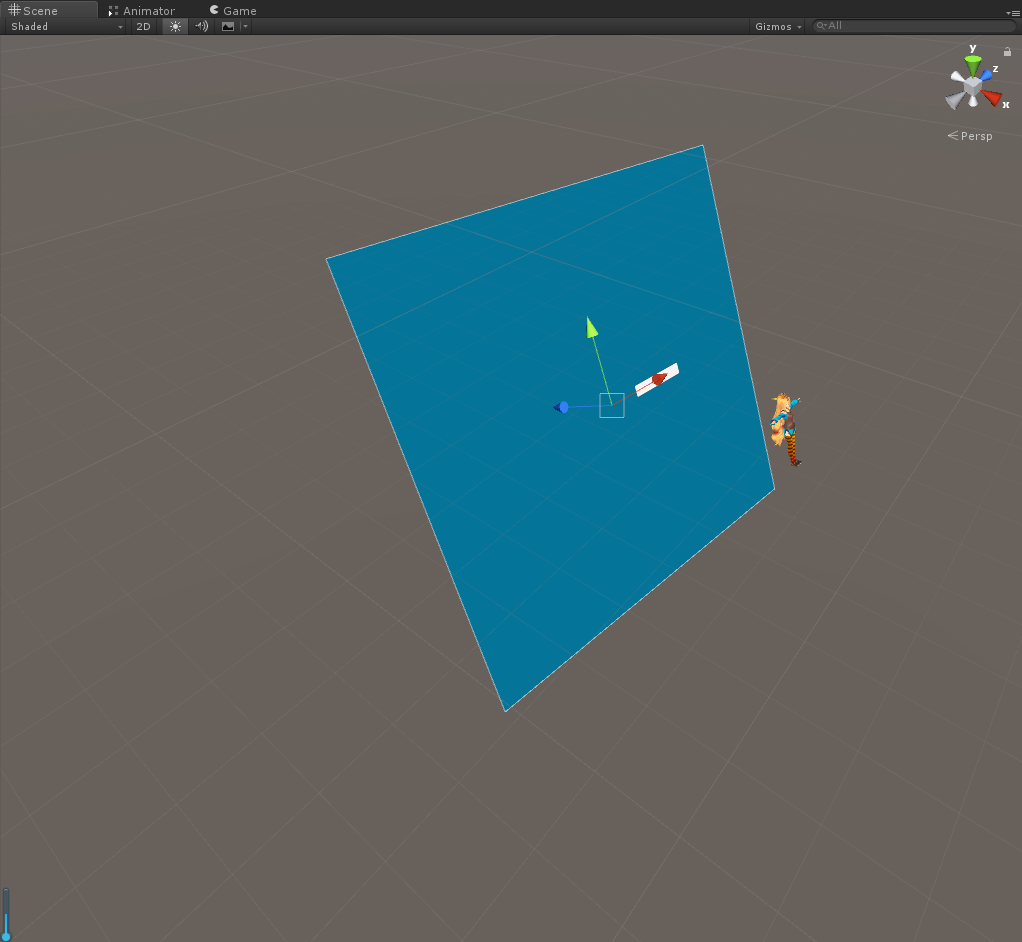
\includegraphics[scale=0.3]{Canva-1.png}
					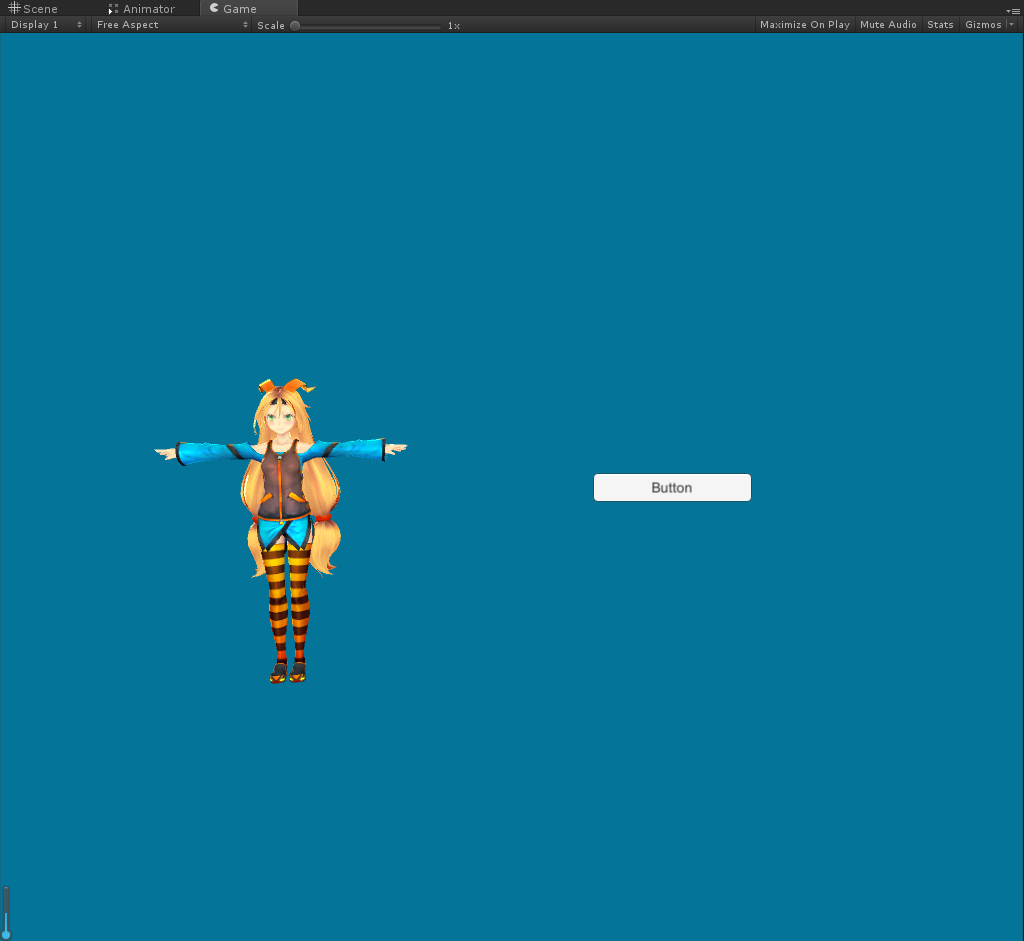
\includegraphics[scale=0.3]{Canvas.png}
					\caption{摄像机模式-画布}
				\end{figure}
			
			它比Screen Space-Overlay模式的画布多了下面几个参数:
				\begin{enumerate}[itemindent = 1em]
					\item \verb|Render Camera|:渲染摄像机
					\item \verb|Plane Distance|:\textbf{画布距离摄像机的距离}
					\item \verb|Sorting Layer|: Sorting Layer是UGUI专用的设置,\textbf{用来指示画布的深度}。可以通过点击该栏的选项,在下拉菜单中点击“Add Sorting Layer”按钮进入标签和层的设置界面,或者点击导航菜单->edit->Project Settings->Tags and Layers进入该页面。
					\item \verb|Order in Layer|:\textbf{在相同的Sort Layer下的画布显示先后顺序。}数字越高,显示的优先级也就越高。
				\end{enumerate}
			
		\subsection{World Space -世界空间模式}
			World Space即世界空间模式。在此模式下,\textbf{画布被视为与场景中其他普通游戏对象性质相同的类似于一张面片(Plane)的游戏物体}。
			
			画布的尺寸可以\textbf{通过RectTransform设置},所有的UI元素可能位于普通3D物体的前面或者后面显示。\textbf{当UI为场景的一部分时,可以使用这个模式}。
			
				\begin{figure}[H]
					\centering
					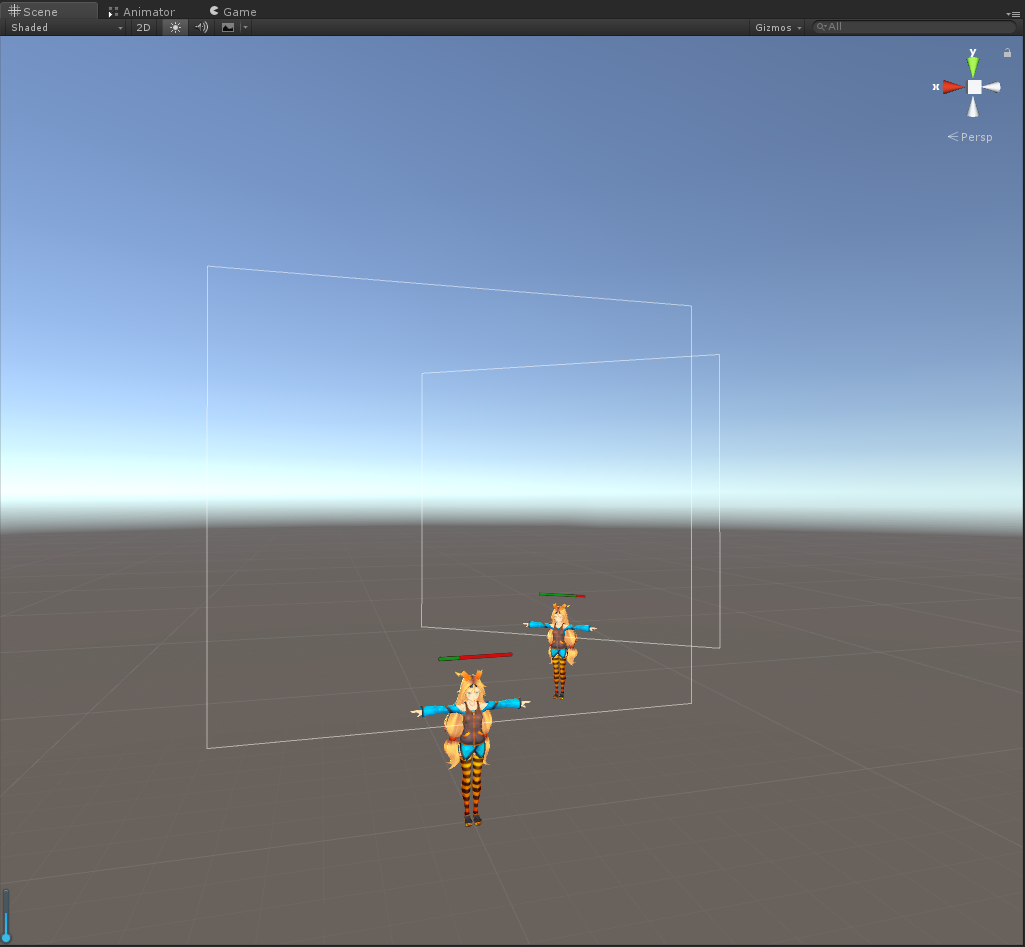
\includegraphics[scale=0.3]{Canvas-2.png}
					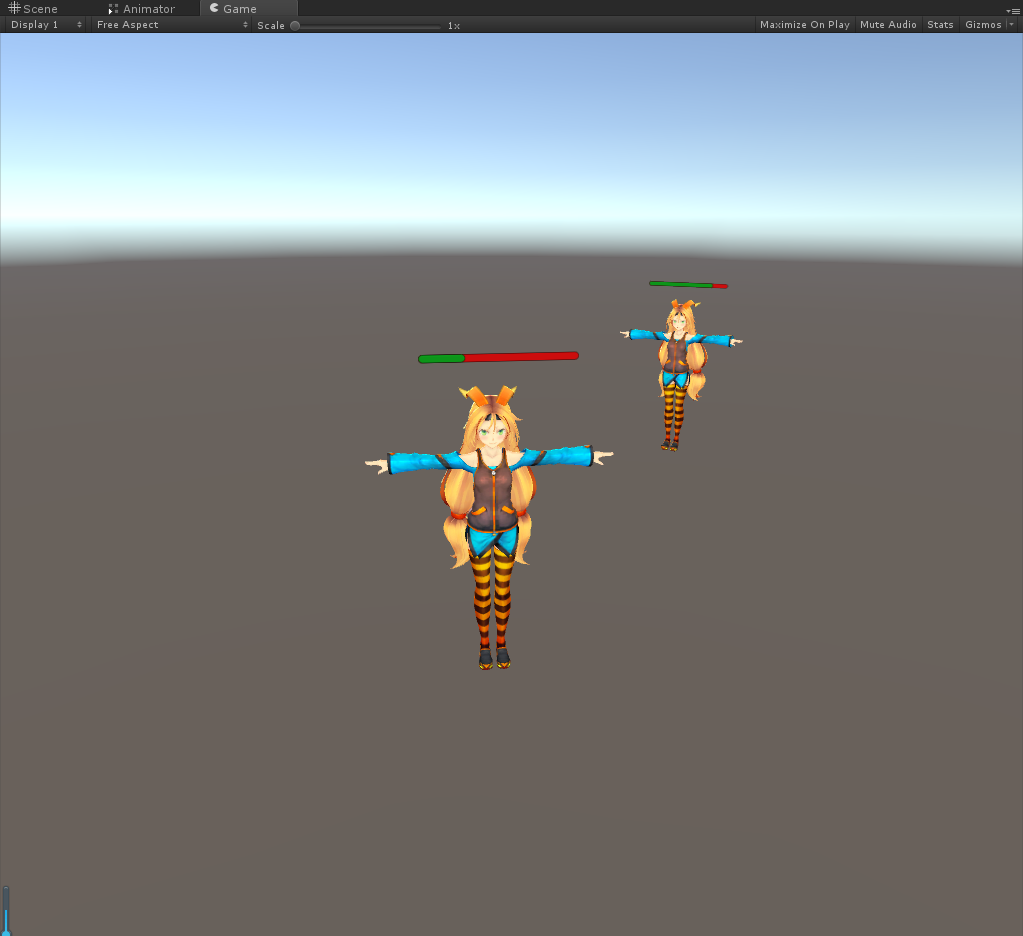
\includegraphics[scale=0.3]{Canvas-3.png}
					\caption{世界空间 模式- 画布}
				\end{figure}
			
		
		\subsection{使用总结}
			\begin{table}[H]
				\centering
				\caption{渲染模式使用场景说明}
				\begin{tabular}{p{4cm}<{\centering}|c|c|c|p{3cm}<{\centering}}
					\toprule
						渲染模式 & 画布匹配屏幕?& 摄像机? & 像素对应 & 适应\\
					\midrule
						覆盖-overlay模式 & 是	& 不需要	& 可选 & 2D \\
						摄像机-camera模式 & 是	& 需要	 & 可选 & 2D+3D\\
						世界空间-world模式 & 否	& 需要	 & 不可选 & 3D\\
					\bottomrule
				\end{tabular}
			\end{table}
		
		\subsection{Canvas Scalar}
			\url{https://blog.csdn.net/qq168213001/article/details/49744899}
		
		\subsection{Layer}
		
		
	\section{RectTransform}
		\url{https://blog.csdn.net/jk823394954/article/details/53861539}
	
		\url{https://blog.csdn.net/rickshaozhiheng/article/details/51569073}
		
		\url{https://blog.csdn.net/serenahaven/article/details/78826851}
		
		核心看:\url{https://blog.csdn.net/Happy_zailing/article/details/78835482}
		
		\url{http://lib.csdn.net/article/unity3d/36875}
		
		RectTransform继承自Transform, 又增加锚点、中心轴点等信息,\textbf{主要提供一个矩形的位置、尺寸、锚点和中心信息以及操作这些属性的方法},\textit{同时提供多种基于父级RectTransform的缩放形式}。
		
		\subsection{Pivot(中心)}
			Pivot用来指示一个\verb|RectTransform|(或者说是矩形)的中(重)心点。	
	
		\subsection{锚点- 自适应屏幕}
			\url{http://www.bubuko.com/infodetail-2384845.html}
			
			
			锚点(四个)由\verb|两个Vector2|的向量确定,这两个向量确定两个点,归一化坐标分别是\verb|Min|和\verb|Max|,\textbf{再由这两个点确定一个矩形},\textbf{这个矩形的四个顶点就是锚点}。
			
			在\verb|Hierarchy|下新建一个Image,查看其\verb|Inspector|。
			
			\begin{figure}[H]
				\centering
				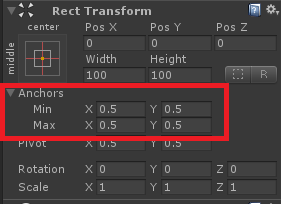
\includegraphics[scale=1.2]{Anchor.png}
				\caption{Anchor 属性}
			\end{figure}
			
			在Min的x、y值分别小于Max的x、y值时,
			\verb|Min |确定矩形\textbf{左下角}的归一化坐标,\verb|Max |确定矩形\verb|右上角|的归一化坐标。
			
			刚创建的Image,其\verb|Anchor的默认值 |为\verb|Min(0.5,0.5)|和\verb|Max(0.5,0.5)|。也就是说,\verb|Min和Max|重合了,四个锚点合并成一点。锚点在Scene中的表示如下:
			
			\begin{figure}[H]
				\centering
				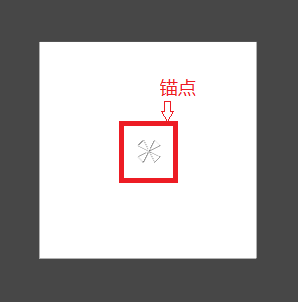
\includegraphics[scale=0.7]{anchorFirst.png}
				\caption{锚点初始位置}
			\end{figure}
		
			将Min和Max的值分别改为\verb|(0.4,0.4)|和\verb|(0.5,0.5)|。可以看见四个锚点已经分开了。
			
			\begin{figure}[H]
				\centering
				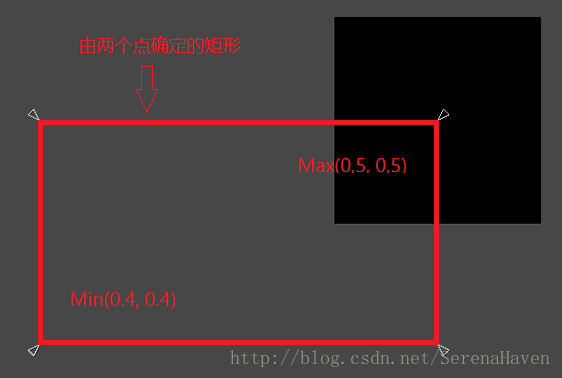
\includegraphics[scale=0.5]{anchorChange.png}
				\caption{min Max位置、确定矩形}
			\end{figure}
			
			
			\subparagraph{需要注意} 在不同的Anchor设置下,控制该RectTransform的变量是不同的。
			
			比如设置成全部居中(默认)时,属性里包含熟悉的用来描述位置的\verb|PosX、PosY和PosZ|,以及用来描述尺寸的\verb|Width和Height|;
			
			切换成全部拉伸时,属性就变成了\verb|Left、Top、Right、Bottom|和\verb|PosZ|,\textbf{前四个属性}用来描述该RectTransform\textbf{分别离父级各边的距离},PosZ用来描述该RectTransform在世界空间的Z坐标
			
			\paragraph{锚点类型}
				\begin{itemize}
					\item 位置类型\verb| 左上角、中心等|
					\item 拉伸类型\verb| 纵向拉伸适配、横向、整体|
				\end{itemize}
		
				\subparagraph{锚点在一块的时候}
					\begin{itemize}[itemindent = 2em]
						\item Anchor 是打在父级窗体上的
						\item Anchor 的位置在父级窗体上的标记方式是按照百分比记录的,单位(百分比)
						\item Anchor 的\verb|Min(RectTransform.anchorMin)  Max(RectTransform.anchorMax)|的信息保持一致
						\item 子物件的 坐标系 为纵向Y,横向X, 并且以\verb|Anchor| 为原点, 自身坐标用中心轴点\verb|Pivot| 表示						
						\item 子物件的 Pivot 与 Anchor  位置始终保持不变,单位(像素)
					\end{itemize}
				
				\subparagraph{锚点单向(横或者纵)分开的时候}
					\begin{itemize}[itemindent = 2em]
						\item 分开的部分(拉伸方向)与父级窗体保持一致变化,单位(百分比)
						\item 与相对方向则绝对保持,单位(像素)
					\end{itemize}
				
				\subparagraph{锚点双向分开的时候}
					\begin{itemize}[itemindent = 2em]
						\item 双向 都与 父级窗体 保持一致的变化,单位(百分比)
						\item 上-top、下-bottom、左、右边距绝对保持,单位(像素)
					\end{itemize}
		
			\paragraph{anchorMax、anchorMin}
				\verb|anchorMin.x|表示锚点在\verb|x|轴的起始点位置,\verb|anchorMax.x|表示锚点在x轴的终点位置,取值\verb|0~1|,表示\textbf{百分比值},该值乘以父窗口的\verb|width|值就是实际锚点相对于父窗口x轴的位置。y轴与x轴同理。
		
					\begin{figure}[H]
						\centering
						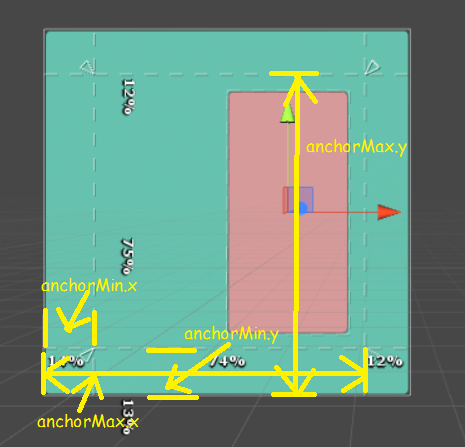
\includegraphics[scale=0.8]{Anchors-3.png}
						\caption{Anchor.Min 与 Anchor.Max}
					\end{figure}
		
				这个值确定了锚点相对于父窗口的位置,是\textbf{真正决定锚点位置的值}
				
			\paragraph{offsetMax 和 offsetMin 属性}
				\subparagraph{锚点 分开时}
					在锚点分开的状态下: 锚点其实是四个钉子,分为左上,左下,右下及右上四个,每个空间在UI模型中都是一个矩形,也有左上,左下,右下及右上四个顶点,那么锚点的每个钉子可以关联一个点,即左上————左上;左下————左下;右下————右下;右上————右上。这样进行绑定。
					
					\verb|offsetMax |是RectTransform\textbf{右上角相对于右上Anchor的距离};
			
					\verb|offsetMin |是RectTransform\textbf{左下角相对于左下Anchor的距离}。
			
					\verb|offset |可以认为是以像素为单位。
					
					\begin{figure}[H]
						\centering
						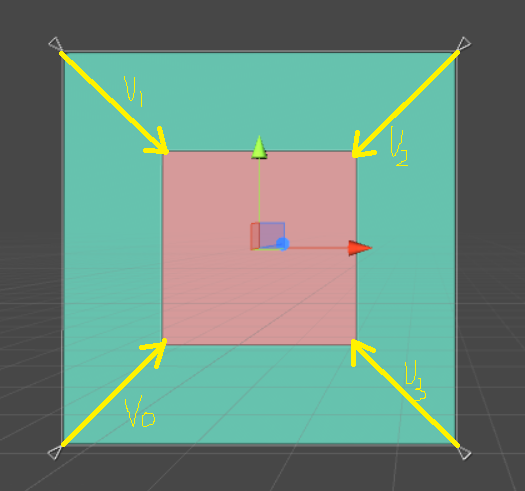
\includegraphics[scale=0.7]{Anchors-1.png}
						\caption{锚点在一起时  Offset 求取向量示例}
						\label{锚点分开时 Offset 求取向量示例}
					\end{figure}
			
				\subparagraph{锚点 在一处时}
					锚点offset 计算如下:
					
					\begin{figure}[H]
						\centering
						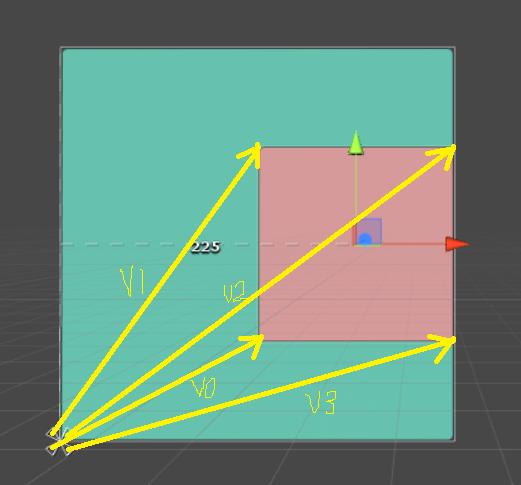
\includegraphics[scale=0.7]{Anchors-2.png}
						\caption{锚点分开时  Offset 求取向量示例}
					\end{figure}
			
				\subparagraph{求取}
					首先计算锚点的每个钉子到其对应的顶点矢量值,分别记作\verb|v0|,\verb|v1|,\verb|v2|,\verb|v3|, 入上图。
					
					然后比较四个向量的\verb|x|值,将\verb|x|的最大值赋给\verb|offsetMax.x|,将\verb|x|的最小值赋给\verb|offsetMin.x|;\verb|y|的值同理。
			
			\paragraph{anchoredPosition}
				\subparagraph{锚点 在一处时}
					anchorPosition 就是 \textbf{从锚点}到本物体的\textbf{轴心}(Pivot)的\textbf{向量值}.
				
				\subparagraph{锚点 分开时}
						
		\subsection{sizeDelta}
		
			\verb|sizeDelta|是\verb|offsetMax-offsetMin|的结果。在\textit{锚点全部重合的情况下},它的值就是面板上的\verb|(Width,Height)|。
			
			\textit{在锚点完全不重合}的情况下,它是相对于父矩形的尺寸。
			
			一个常见的错误是,当RectTransform的锚点\textbf{并非全部重合时},使用sizeDelta作为这个RectTransform的尺寸。此时拿到的结果一般来说并非预期的结果。
			
		\subsection{RectTransform.rect}	
			RectTransform.rect 的各值如图所示。
			
			\begin{figure}[H]
				\centering
				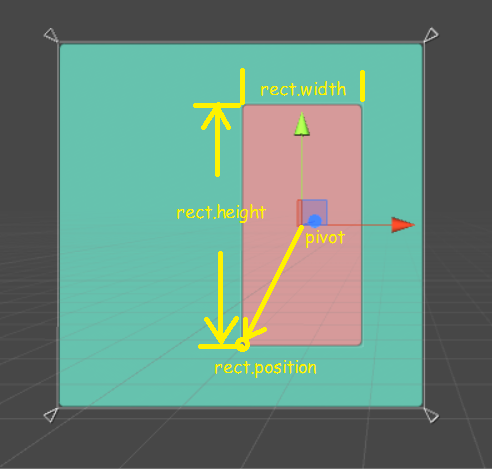
\includegraphics[scale=0.8]{RectTransform-rect.png}
				\caption{RectTransform rect 属性}
			\end{figure}	
		
		\subsection{示例}
			\begin{lstlisting}
	GameObject webText = new GameObject("webText");
	webText.AddComponent<UnityEngine.UI.Text>();
	webText.GetComponent<UnityEngine.UI.Text>().text = "";
	webText.GetComponent<RectTransform>().anchorMin = new Vector2(0, 0);
	webText.GetComponent<RectTransform>().anchorMax = new Vector2(1, 1);
	webText.GetComponent<RectTransform>().sizeDelta = new Vector2(0, 0);
	webText.GetComponent<RectTransform>().anchoredPosition = new Vector2(0, 0);
	webText.transform.localPosition = new Vector3(0,0,0);
	webText.transform.SetParent(webObj.transform, false);
			\end{lstlisting}
			
		\subsection{FramDebug}
			查看渲染的先后顺序
			
			\verb|windows->FrameDebug |	
	\section{按钮}
		\subsection{RayCast Target-点击事件的获取原理}
			参考文献:\url{https://blog.csdn.net/liujunjie612/article/details/55097789}
			
			UGUI会遍历屏幕中所有RaycastTarget是true的UI,接着就会发射线,并且排序找到玩家最先触发的那个UI,在抛出事件给逻辑层去响应。
			
			团队多人在开发游戏界面,很多时候都是复制黏贴,比如上一个图片是\textbf{需要响应}RaycastTarget,然后ctrl+d以后复制出来的也就带了这个属性,很可能新复制出来的图片是\textbf{不需要响应的},开发人员\textbf{又没有取消勾选掉},\textit{这就出问题了}。
			
			所以RaycastTarget如果被勾选的过多的话, 效率必然会低。
		\subsection{原始Button}
			
		\subsection{Image等 -添加button 组件}
			\begin{itemize}
				\item \verb|create -> UI -> Image|
				\item \verb|Inspirit -> Add Component -> button|
			\end{itemize}	
		
		\subsection{添加事件处理脚本}
			\begin{itemize}
				\item 书写脚本并添加到Button gameObject 上
				\item 如果是Button 组件的话直接在button 组件上添加,如果是Image 则添加button 组件后再添加
				\item  添加脚本对象到\verb|onClick() |部分:\verb|+ -> gameObject 拖进来  -> 选择脚本中的具体函数|
			\end{itemize}
		
	\section{文本- Text}
		\subsection{添加文字阴影 -shadow 组件}
			\verb|addComponent -> shadow|
			
		\subsection{添加文子边框 -outline 组件}
			\verb|addComponent -> outline|
			
	\section{图片- ImageView}
		
	\section{选中标记- Toggle}
		\paragraph{Toggle 基本}
		
		\paragraph{Toggle Group}
			\subparagraph{选项栏设定}
				将panel  拖入 toggle 中的\verb|value changed|部分
				
			\subparagraph{预设}
				确定默认打开哪个panel,然后将其\verb|IsOn| 勾选,其余取消勾选	
				
	\section{滚动区域、滚动条}
	
	
	\section{其他工具条}
	
	\section{布局- Layout}
		\begin{itemize}
			\item 具体页面下创建空物体 \verb| GameObject|
			\item 其次在\verb|GameObject 下|添加组件 \verb|-> grid layout group|
			\item 最后在这个\verb|GameObject |下创建出各种Image 组件,然后这些组件将会以\verb|grid layout| 的布局进行自动调整
		\end{itemize}
	
		\subsection{grid layout group}
			\begin{itemize}
				\item  调整\verb|cell size| 进行调整子物件的大小
				\item  \verb|cell size| 的改变只影响子组件的第一层,既最下面一层
			\end{itemize}
		
		\subsection{horizontal layout group}
		
		\subsection{vertical layout group}

\chapter{物理}
	\section{流程}
		\begin{itemize}
			\item \verb|RigidBody |:创建,以完成受力接收。
			\item \verb|Physical Material|:创建,以完成多种力的添加。
			\item \verb|Material |:拖入材质球。
		\end{itemize}
	
	\section{刚体}
	
	
	\section{碰撞器}
	
	
	\section{物理材质}
	
	
	\section{触发器}
	
	
	\section{射线}
	
	
	\section{关节}
		
\chapter{动画}
	\section{流程}
		\dirtree{%
			.1 .
			.2 在要动态显示的物体的父节点上创建\textbf{Animation} .
			.3 编辑Animation .
			.4 在脚本中获取该父亲节点上的Animator 组件 .
			.5 播放动画 .
		}
		
		
	
	\section{iTween 动画用法}
		

\chapter{粒子系统}

		
\chapter{着色器}
	入门参考网址:\url{https://blog.csdn.net/ring0hx/article/details/46440037}
	
	\section{Shader 版本}
		Shader 1.0(DirectX8.0)、
		Shader 2.0(DirectX9.0b)、
		Shader 3.0(DirectX9.0c)、
		Shader 4.0(DirectX10)、
		Shader 4.1(DirectX10.1)
		和Shader 5(DirectX11)。

		\begin{figure}[H]
			\centering
			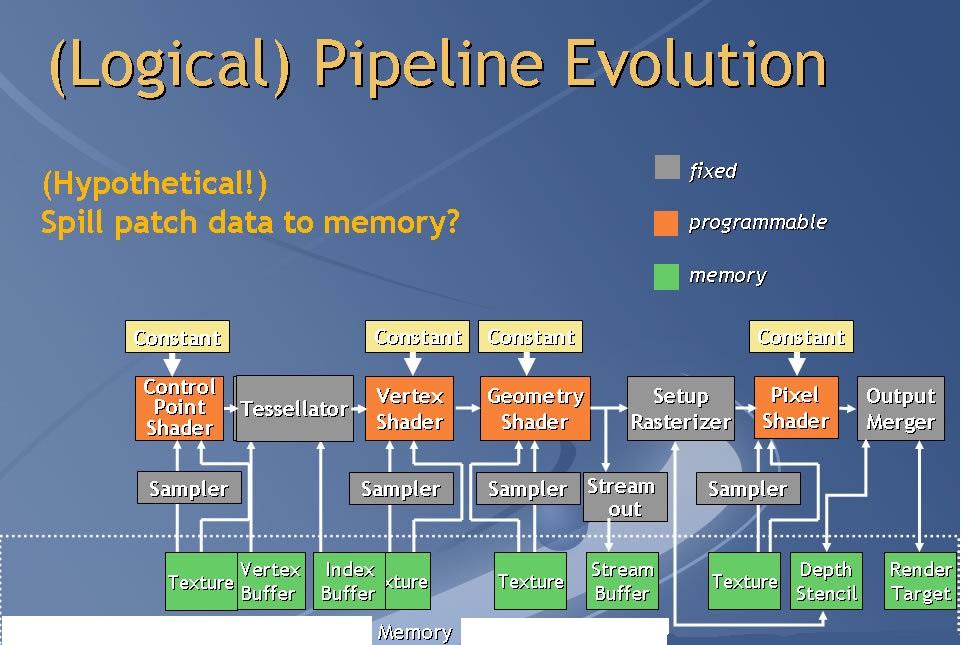
\includegraphics[scale=0.71]{ShaderArc}
			\caption{shader  通用架构}
		\end{figure}
		
		
	\section{结构}
		\begin{figure}[H]
			\centering
			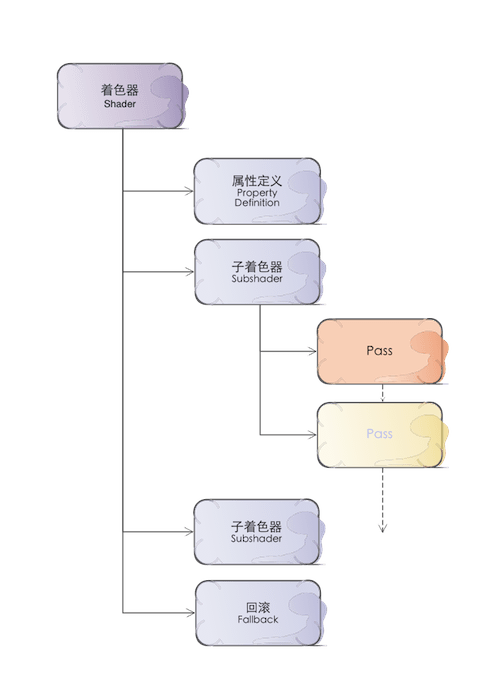
\includegraphics[scale=0.8]{arch}
			\caption{着色器结构}
		\end{figure}
		
		\begin{itemize}
			\item \textbf{属性定义(Property Definition)}:定义Shader的输入,并且绑定到编辑器上。
			\item \textbf{子着色器(SubShader)}:\underline{一个Shader可以有多个子着色器。}这些子着色器互不相干且\textbf{只有一个会在最终的平台运行}。\textit{编写多个的目的是解决兼容性问题。Unity会自己选择兼容终端平台的Shader运行}。
			\item \textbf{回滚(Fallback)}:如果子着色器在终端平台上都无法运行,那么使用Fallback指定的备用Shader,\textbf{俗称备胎}。
			\item \textbf{Pass}:\textit{一个Pass就是一次绘制}。\textbf{对于表面着色器,只能有一个Pass},所以不存在Pass节。\textbf{顶点片段着色器可以有多个Pass。}多次Pass可以实现很多特殊效果,例如当人物被环境遮挡时还可以看到人物轮廓就可以用多Pass来实现。
			\item \textbf{Cg代码}:每个Pass中都可以包含自定义的Cg代码,\textbf{从CGPROGRAM开始到ENDCG结束}。
		\end{itemize}
	\section{Shader2.0}
		可以实现编程。
		
		\url{https://www.cnblogs.com/lixiang-share/p/5025662.html}
		
		\paragraph{大概流程}
			\dirtree{%
				.1 .
				.2 MeshRender 将CPU数据传入至GPU .
				.3 然后传递给顶点着色器 .
				.4 顶点着色器处理完成后,将自己的输出数据传递给 片段着色器处理 .
			}

		
		\paragraph{定义顶点着色器入口函数}
			\verb|#pragma vertex _vertexFunctionName |
			
		\paragraph{定义片段着色器入口函数}
			\verb|#pragma fragment _fragmentFunctionName |

		\paragraph{定义平面着色器入口函数}
			\verb|#pragma surface _surfaceFunctionName |
			
		
		\paragraph{常用语义}
			POSITION\textbf{语义}等相当于告诉渲染引擎,这个变量是代表什么含义。
			
			\begin{itemize}
				\item \verb|POSITION| 获取模型顶点信息。
				\item \verb|NORMAL| 获取法线信息。
				\item \verb|TEXCOORD n| 第(n)张贴图的uv坐标
				\item \verb|COLOR n| 第n个定点色。\verb|float4|
				\item \verb|TANGENT| 获取切线信息
				\item \verb|SV_POSITION| 表示经过MVP 矩阵已经转化到屏幕坐标的位置
				\item \verb|SV_TARGET| 输出到哪个Render Target 上
 			\end{itemize}
		
		\paragraph{常用坐标系}
			\begin{itemize}
				\item \verb|模型坐标系|:也叫物体坐标系,3D建模的时候每个模型都是在自己的坐标系下建立的,如果一个人物模型脚底是(0,0,0) 点的话它的身上其它点的坐标都是相对脚底这个原点的。 
				\item \verb|世界坐标系|:我们场景是一个世界,有自己的原点,模型放置到场景中后模型上的每个顶点就有了一个新的世界坐标。这个坐标可以通过模型矩阵×模型上顶点的模型坐标得到。 
				\item \verb|视图坐标系|:又叫观察坐标系,是以观察者(相机)为原点的坐标系。场景中的物体只有被相机观察到才会绘制到屏幕上,相机可以设置视口大小和裁剪平面来控制可视范围,这些都是相对相机来说的,所以需要把世界坐标转换到视图坐标系来方便处理。 
				\item \verb|投影坐标系|:场景是3D的,但是最终绘制到屏幕上是2D,投影坐标系完成这个降维的工作,投影变换后3D的坐标就变成2D的坐标了。投影有平行投影和透视投影两种,可以在Unity的相机上设置。 
				\item \verb|屏幕坐标系|: 最终绘制到屏幕上的坐标。屏幕的左下角为原点。
			\end{itemize}

		\paragraph{常用矩阵表示}
			\begin{itemize}
				\item \verb|UNITY_MATRIX_MVP|:当前模型 -> 视图 -> 投影矩阵。(注:模型矩阵为 本地->世界)
				\item \verb|UNITY_MATRIX_MV|:当前模型 -> 视图矩阵
				\item \verb|UNITY_MATRIX_V|:当前视图矩阵
				\item \verb|UNITY_MATRIX_P|:当前投影矩阵
				\item \verb|UNITY_MATRIX_VP|:当前视图 -> 投影矩阵
				\item \verb|UNITY_MATRIX_T_MV|:转置模型 -> 视图矩阵
				\item \verb|UNITY_MATRIX_IT_MV|:逆转置模型 -> 视矩阵, 用于将法线从\verb|ObjectSpace|旋转到\verb|WorldSpace|。为什么法线变化不能和位置变换一样用\verb|UNITY_MATRIX_MV|呢?一是因为法线是3维的向量而- \verb|UNITY_MATRIX_MV|是一个4x4矩阵,二是因为法线是向量,我们只希望对它旋转,但是在进行空间变换的时候,如果发生非等比缩放,方向会发生偏移。
				\item \verb|UNITY_MATRIX_TEXTURE0 |to \verb|UNITY_MATRIX_TEXTURE3|:纹理变换矩阵
			\end{itemize}
			
	\section{材质、贴图、纹理}
			材质 Material包含贴图 Map,贴图包含纹理 Texture。
			
			\paragraph{纹理}\verb|->|
			
				是最基本的数据输入单位,游戏领域基本上都用的是位图。常见格式有PNG,TGA,BMP,TIFF此外还有程序化生成的纹理 Procedural Texture。 
				在内存中通常表示为二维像素数组。
				
			\paragraph{贴图}\verb|->|
			
				英语 Map 其实包含了另一层含义就是“映射”。其功能就是\underline{把}\textbf{纹理}通过 \verb|UV 坐标| \underline{映射}到 \textit{3D 物体表面}。
				
				\textbf{贴图}\textit{包含了}\textbf{除了纹理以外其他很多信息},比方说 \textbf{UV 坐标}、\textbf{贴图输入输出控制}等等。 
				一张图便能说明其之间的关系 
				\begin{figure}[H]
					\centering
					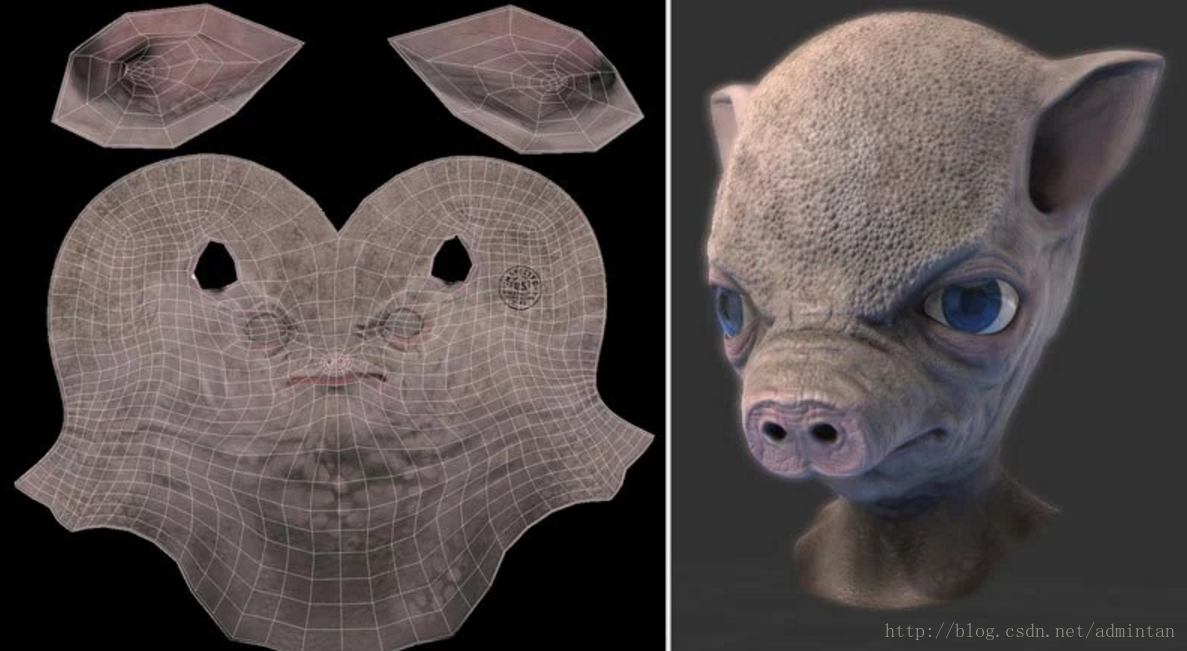
\includegraphics[scale=0.57]{Texture}
					\caption{纹理与贴图}
				\end{figure}
				
			\paragraph{材质}\verb|->|
			
				本质就是一个\textbf{数据集},主要功能就是\textbf{给渲染器}\textit{提供数据和光照算法}。
				
				\textbf{贴图}就是其中\textbf{数据的一部分},根据用途不同,贴图也会被分成不同的类型,比方说 \verb|Diffuse Map|,\verb|Specular Map|,\verb|Normal Map| 和 \verb|Gloss Map| 等等。
				
				\textbf{另外一个重要部分}就是\textbf{光照模型 Shader} ,用以实现不同的渲染效果。 贴图种类繁多:我做个不完全总结
				
				\subparagraph{Diffuse Map}
					漫反射贴图/也被称作反照率贴图albedo map, 存储了物体相应部分漫反射颜色
					
				\subparagraph{Normal Map}
					法线贴图 本质上存储的是被RGB值编码的法向量 表现凹凸,\textbf{比如一些凹凸不平的表面,光影在表面产生实时变化,常用来低精度多边形表现高精度多边形细节}, \textbf{比如在高多边形下生成normal map在匹配给低多边形模型 是一种常见的降低性能要求的做法}
					
					\begin{figure}[H]
						\centering
						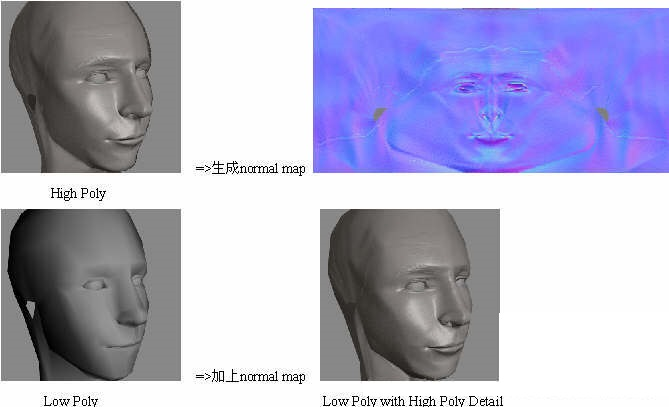
\includegraphics[scale=0.8]{normalMap}
						\caption{法线贴图演示}
					\end{figure}
					
					建议参考:\url{https://blog.csdn.net/cywater2000/article/details/749341#comments}
					
					常规来说就是\textbf{光向量}和\textbf{法向量}的\textbf{点积}\textit{来确定明暗以表现凹凸质感},也就是把法线存在纹理中。
				\subparagraph{Specular Map}
					高光贴图 表现质感 高光区域大小可真实反映材质区别
					
				\subparagraph{Gloss Map}
					光泽贴图,每个纹理元素上描述光泽程度
					
			总体上说 他们都是要被shader加工的原材料.
	
	\section{光照模型}
		参考:\url{https://blog.csdn.net/admintan/article/details/53913624}
		
		\subsection{Phone 光照模型}
			真实世界中的光照效果抽象为三种独立的光照效果的叠加。
				$$Color = Ambient + Diffuse + Specular$$
			
			\paragraph{环境光-Ambient}
				此为模拟环境中的整体光照水平,是间接反射光的粗略估计,间接反射的光使阴影部分不会变成全黑 关于环境光还有个事实,1某个可以独立分析的局部场合的环境光强和能够进入这个地方的光的强度有关。 
					
					$$Ambient = K_a * GlobalAmbient $$
					
			\paragraph{漫反射光-Diffuse}
				模拟直接光源在表面均匀的向各个方向反射,能够逼近真实光源照射到哑光表面的反射。比如在阳光下,由于路面粗糙的性质,我们发现从任意一个角度观察路面,亮度都是差不多。 
				
					$$Diffuse = K_d * lightColor * dot(L,N) $$
			\paragraph{镜面反射光-Specular}
				模拟在光滑表面会看到的光亮高光。会出现在光源的直接反射方向。镜子、金属等表面光亮的物体会有镜面反射光。镜面反射光同时与物体表面朝向、光线方向、视点位置有关。如图:
					\begin{figure}[H]
						\centering
						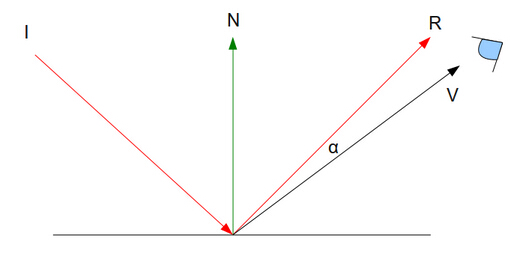
\includegraphics[scale=0.8]{Specular}
						\caption{高光演示}
					\end{figure}
				
				$I$是入射光,$N$是表面法线,$R$是反射光线,$V$是从物体上的目标观察点指向视点的向量,$a$是$V$和$R$的夹角。
				
				我们可以判断出一个规律,夹角$a$越小,即视线与反射方向的偏离越小,则目标点的光强越大,计算公式为:
					
					$$Specular = K_s * lightColor * (dot(V,R))^{shininess}$$ 
				
					\begin{itemize}
						\item Ks为物体对于反射光线的衰减系数
						\item Shininess为高光指数,高光指数反映了物体表面的光泽程度。
						\begin{itemize}
							\item Shininess越大,反射光越集中,当偏离反射方向时,光线衰减的越厉害,只有当视线方向与反射光线方向非常接近时才能看到镜面反射的高光现象,此时,镜面反射光将会在反射方向附近形成亮且小的光斑;
							\item Shininess 越小,表示物体越粗糙,反射光分散,观察到的光斑区域小,强度弱。
						\end{itemize}
					\end{itemize}
			
			\paragraph{总结}
				至于更多的光照模型结合了更多的物理光学等信息 在模拟单种材质例如塑料 合金 石膏陶瓷等等上要好于Phone式模型的效果 但是基本上属于Phone式模型的扩充
				
				
\chapter{资源管理- AssetBundle}
	\section{工作流程}
		\dirtree{%
			.1 \textbf{AssetBundle 的使用流程} . 
			.2 1- 创建AssetBundle .
			.3 2- 上传到Server .
			.4 3- 游戏运行时根据需要下载AssetBundle 文件 .
			.5 4- 解析加载Assets .
			.6 5- 使用完后释放内存等资源 .
		}
	\section{创建}
		通过编译管线BuildPipeline来创建AssetBundle文件,总共有三种方法,具体如下所示。
		\subsection{BuildAssetBundle}
			该API将编辑器中的任意类型的Assets打包成一个AssetBundle,适用于\textbf{对单个大规模场景的细分}。
			
			\begin{itemize}
				\item 名称:\textbf{BuildPipeline.BuildAssetBundle}
				\item 参数-1:\textbf{mainAsset} : Object
				\item 参数-2:\textbf{assets} : Object[]
				\item 参数-3:\textbf{pathName} : string
				\item 参数-4:\textbf{options} : BuildAssetBundleOptions
				\item 参数-5:\textbf{targetPlatform} : BuildTarget = BuildTarget.WebPlayer
				\item 返回值:\textbf{bool}
			\end{itemize}
			
			\paragraph{BuildAssetBundleOptions}
				\subparagraph{CompleteAssets}
				
				\subparagraph{CollectDependencies}
				
				\subparagraph{DisableWriteTypeTree}
				
				\subparagraph{DeterministricAssetBundle}
				
				\subparagraph{UncompressedAssetBundle}

			\paragraph{AssetBundle之间的依赖}	
				如果游戏中的某个资源被多个资源引用(例如游戏中的Material),单独创建AssetBundle会使多个AssetBundle都包含被引用的资源(这里跟flash编译选项中的链接选项有些像),从而导致资源变大,这里可以通过指定AssetBundle之间的依赖关系来减少最终AssetBundle文件的大小(把AssetBundle解耦)。
				
				具体方法是在创建AssetBundle之前调用BuildPipeline.PushAssetDependencies和BuildPipeline.PopAssetDependencies来创建AssetBundle之间的依赖关系,它的用法就是一个栈,后压入栈中的元素依赖栈内的元素。
			
		\subsection{BuildStreamedSceneAssetBundle}
			该API将一个或多个场景中的资源及其所有依赖以流加载的方式打包成AssetBundle,一般适用于\textbf{多单个或多个场景进行集中打包}
			
			\begin{itemize}
				\item 名称:\textbf{BuildPipeline.BuildStreamedSceneAssetBundle}
				\item 参数-1:\textbf{level} : string[]
				\item 参数-2:\textbf{locationPath} : string
				\item 参数-3:\textbf{target} : BuildTarget
				\item 返回值:\textbf{String}
			\end{itemize}

			
			
		\subsection{BuildAssetBundleExplicitAssetNames}
			该API功能与a相同,但创建的时候可以为每个Object指定一个自定义的名字。(一般不太常用)
			
			\begin{itemize}
				\item 名称:\textbf{BuildPipeline.BuildAssetBundleExplicitAssetNames}
				\item 参数-1:\textbf{assets} : Object[]
				\item 参数-2:\textbf{assetNames} : string[]
				\item 参数-3:\textbf{pathName} : string
				\item 参数-4:\textbf{options} : BuildAssetBundleOptions
				\item 参数-5:\textbf{targetPlatform} : BuildTarget
				\item 返回值:\textbf{bool}
			\end{itemize}			
		    
	\section{使用}
	
	\section{卸载}
	
	\section{内存模型}
	
	\section{其他}

\chapter{Editor 扩展}
	Unity编辑器扩展是扩展Unity菜单功能,也可以说是自定义Unity菜单,以此来便利我们能够更快捷地开发游戏。
	\section{流程}
		\begin{enumerate}
			\item 在Asset文件夹下\textbf{创建一个文件夹}\verb|Editor|,如果已经存在则忽略此步
			\item 在\verb|该Editor| 文件夹下,\textbf{创建一个}\verb|C#|\textbf{脚本},无需继承于任何类
			\item \textbf{引用}\verb|UnityEditor| \textbf{命名空间}
			\item \textbf{写静态方法}\textit{既菜单的功能},类似于\verb|[SerilizedFiled]|下的东西,与\verb|[Menuitem("Netease/xx")]|一一对应。
			\item \textbf{给该方法上添加}\verb|[Menuitem("")]|特性
		\end{enumerate}	
	
	\section{在编辑器上增加一个MenuItem}
	
	
	\section{创建一个对话框}
	
	
	\section{扩展Inspector面板}
	
	
	
	\section{编辑器插件常用函数}
		\subsection{资源导入回调函数}
			当导入资源到Unity 项目中的某个资源文件夹下时,当Unity Editor获得焦点后,会在加载完资源后,先为其创建.meta 文件,然后再触发该回调函数。
			
			\begin{lstlisting}[frame=line]
	public class TestBundleNameAndTexture : UnityEditor.AssetPostprocessor
	{
	    static void OnPostprocessAllAssets(  // 这个函数必须为静态的,其他可以不是!
	        string[] importedAssets,
	        string[] deletedAssets,
	        string[] movedAssets,
	        string[] movedFromAssetPaths)
	    {
	        foreach (var path in importedAssets)
	        {
	            DirectoryInfo dir = new DirectoryInfo(path);
	            Debug.Log(dir.Parent.FullName);
	            BundelNameCreater.Proc(dir.Parent.FullName);
	        }
	    }
	
	}
			\end{lstlisting}
	\section{一些常用的Inspector属性设置}
	
	
	\section{参考}
		\url{https://blog.csdn.net/puppet_master/article/details/51012298}
		
		\url{http://blog.csdn.net/asd237241291/article/details/38235091}
		
		\url{http://blog.sina.com.cn/s/blog_471132920101n8cr.html}
		
\chapter{跨平台发布apk}
	\section{流程}
		\begin{itemize}
			\item 安装 JavaSDK、Android Studio 并在SDK manager 里添加对应的API包
			\item 在unity 中的\verb|edit |选项下的\verb|preferences|, 并选中\verb|External Tools| 选项,配置\verb|JDK |和\verb|Android SDK| 安装位置。
			\item 在unity 中的\verb|File -> Build Settings|中,添加需要添加的场景,并选择对应的平台(Android, IOS)等
			\item 在unity 中的\verb|Build Settings |中的\verb|Player Settings |设置以下几个重要内容。
				\begin{enumerate}
					\item \verb|Company Name |
					\item \verb|Product Name |
					\item \verb|Default Icon |:192$\times$192
					\item \verb|Default Orientation |
					\item \verb|Other Settings -> Identification |:修改为\verb|com.netease(Or Other).TestName(Or Other)|
				\end{enumerate}
		\end{itemize}	
	
	\section{Apk 安装常见错误}
		\url{http://mumu.163.com/2017/03/30/25905_680657.html}


\chapter{调试技巧}
	\section{以父类为基点}
		在Inspector 中查看是否存在父类脚本\verb|[SerializedField]| 的变量,这样方便对空间进行查找,并且添加新的\textbf{控制}			
	
	
	
\chapter{GPU 相关}
	大部分时间在\textbf{知其然不知其所以然}。该部分将\textit{从GPU讲到游戏引擎再到游戏}逐层介绍,以打通任督2脉。 

	介绍绘画流程的video:\url{https://v.youku.com/v_show/id_XNjY3MTY4NjAw.html}
	
	本节参考:\url{https://blog.csdn.net/admintan/article/details/53861781}
	\section{最底层——GPU/硬件原理}
		
		\subsection{硬件基础}
			\paragraph{ALU-Arithmetic Logic Unit 算数逻辑单元}\verb|->|
			
				整数算术运算(加、减,有时还包括乘和除,不过成本较高)、位逻辑运算(与、或、非、异或)、移位运算(将一个字向左或向右移位或浮动特定位,而无符号延伸),移位可被认为是乘以2或除以 2。 ALU可以说是计算机处理器的核心部件之一。

			\paragraph{Cache-缓存SRAM}\verb|->|
			
				SRAM叫静态内存,“静态”指的是当我们将一笔数据写入SRAM后,除非重新写入新数据或关闭电源,否则写入的数据保持不变。 
				
				由于CPU的速度比内存和硬盘的速度要快得多,所以在存取数据时会使CPU等待,影响计算机的速度。SRAM的存取速度比其它内存和硬盘都要快,所以它被用作电脑的高速缓存(Cache)。
		\subsection{CPU with GPU 异同}
		
			参考:\url{https://www.jianshu.com/p/fae645d70e0e}
		
			\begin{figure}[H]
				\centering
				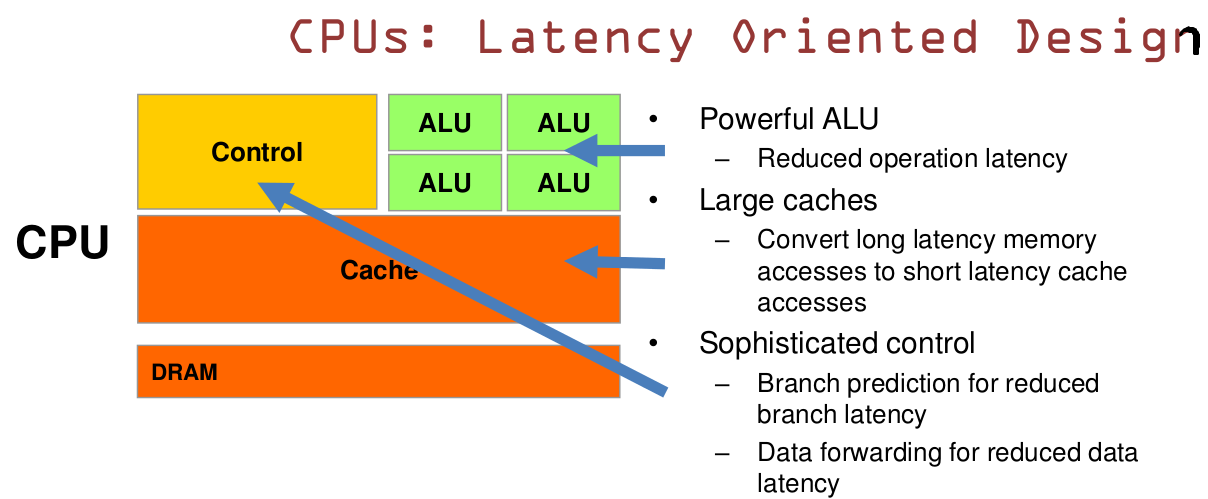
\includegraphics[scale=0.4]{CpuWithGpu}
				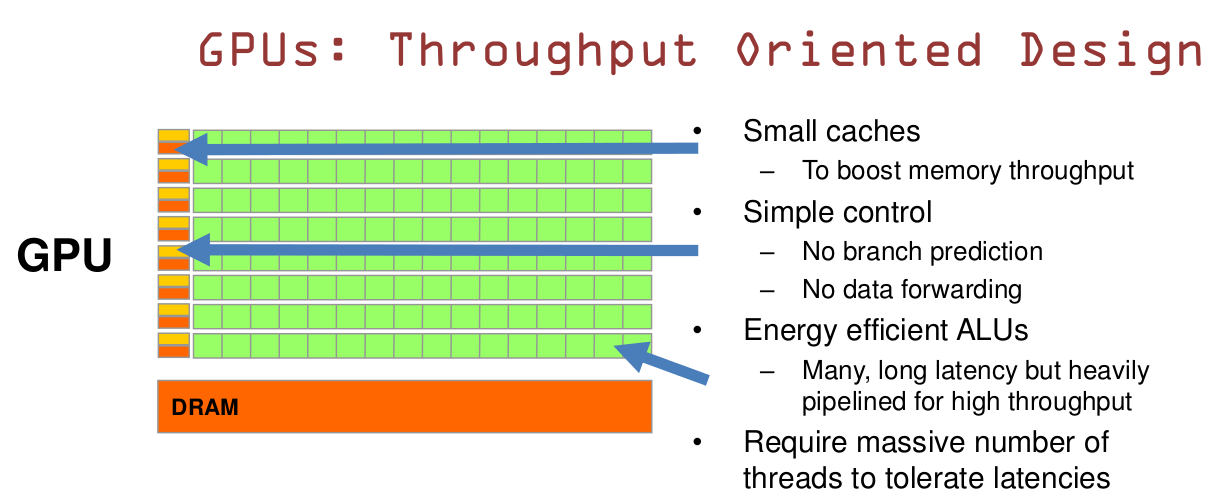
\includegraphics[scale=0.4]{CpuWithGpu2}
				\caption{CPU with GPU}
			\end{figure}
		
			\paragraph{CPU}\verb|->|
					量小但能力强
					\begin{itemize}
						\item 	ALU\textbf{部分会很强大},可以在很少的时钟周期内完成算数计算。 对于一个64bit双精度的CPU来说 浮点加法和乘法只需要1-3个时钟周期。 							
						\item 	\textbf{大的Cache}也将延时降低很多, 结合了现在的各种高级调节技术比如超线程、多核等技术CPU对于复杂逻辑的运算能力得到了极大提升。
					\end{itemize}
			
			\paragraph{GPU}\verb|->|
					量大但能力弱
					\begin{itemize}
						\item ALU的\textbf{数量会非常大}、\textbf{功能会更少}、\textbf{能耗很低}、\textbf{cache就会很小},
						这样带来的好处就是针对大吞吐量的需要简单计算的数据来说,处理效率就高了非常多。
						
						如果有很多线程需要访问同一个相同的数据,\textit{缓存会合并这些访问,然后再去访问DRAM}(因为需要访问的数据保存在DRAM中而不是Cache里面),\textbf{获取数据后Cache会转发这个数据给对应的线程,这个时候是数据转发的角色}。但是由于需要访问DRAM,自然会带来延时的问题。
						
						\item GPU的控制单元(左边黄色区域块)\textbf{可以把多个的访问合并}成少的访问。
						
						\item GPU的虽然有DRAM延时,\textbf{却有非常多的ALU和非常多线程}. 为了平衡内存延时的问题,我们可以中充分利用多的ALU的特性达到一个非常大的吞吐量的效果。尽可能多的分配多的线程.通常来看GPU ALU会有非常重的pipeline就是因为这样。
					\end{itemize}
			
			\paragraph{结论}\verb|->|
			
				我们可以先得出一个简单结论:\color{blue}\textbf{对显卡来说}\color{black}-\textbf{更适合做高并行,高数据密度,简单逻辑的运算}。
	
		\newpage
		\subsection{GPU 架构}
			\paragraph{4D向量 和 4+1}\verb|->|
							
				3D物件的成像過程中,VS(Vertex Shader,\textbf{顶点着色引擎})PS(Pixel Shader,\textbf{像素著色引擎} 或片段着色器)\textbf{最主要的作用就是运算坐标(XYZW)@(RGBA)}。
				
				此时数据的\textbf{基本单位是scalar(标量)},1个单位的变量操作,为1D标量简称1D。 
				而跟标量相對的就是vector(向量),\textbf{向量是由多個标量构成}。\textit{例如每個周期可执行4個向量平行运算,就称为4D向量架构}。若GPU指令发射口只有1个,卻可執行4個数据的平行运算,这就是SIMD(单指令多数据流)架构。	
			
			\paragraph{运算单元计算机制}\verb|->|
				
				以GPU的矩阵加法为例:
				\begin{figure}[H]
					\centering
					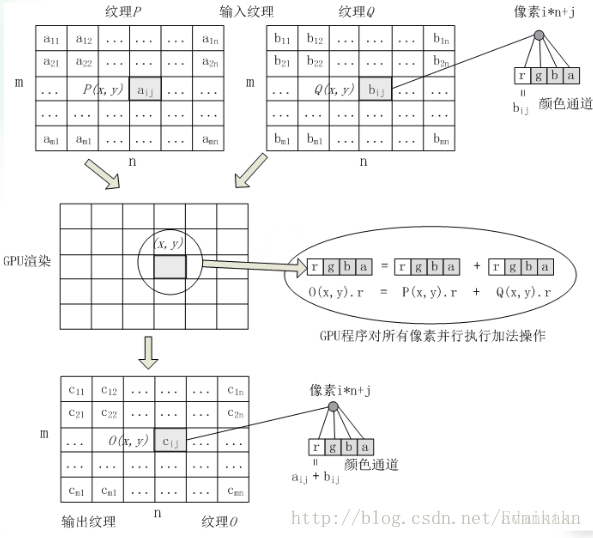
\includegraphics[scale=0.84]{comU}
					\caption{运算单元计算机制}
				\end{figure}

			
			\paragraph{NVIDIA}\verb|->|
			
				NVIDIA架构如下
				\begin{figure}[H]
					\centering
					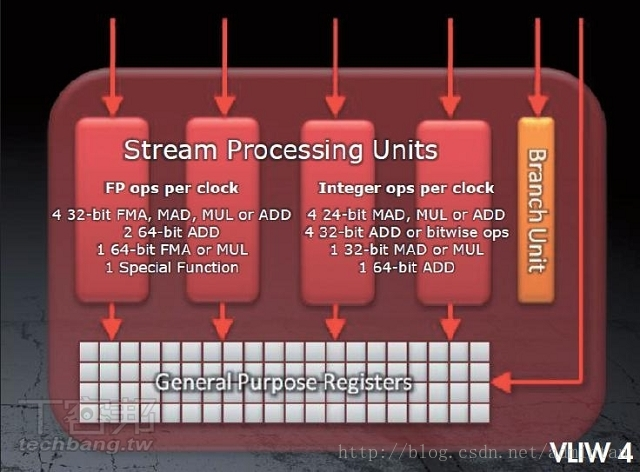
\includegraphics[scale=0.5]{NVIDIA}
					\caption{NVIDIA架构演示}
				\end{figure}
				
				标注的是\verb|Stream Processing|(流处理器)数量, 
				NVIDIA的流处理器每个都具有完整的ALU(可以理解为数学、逻辑等运算)。NVIDIA从G80以后采用全标量设计,\textbf{所有运算全都转为标量计算。但是这么做一旦遇到4D矢量运算时,就需要4次运算才能完成},所以NVIDIA显卡的Shader频率几乎比核心频率高一倍,就是为了弥补这个缺点。 
				NV的流处理器都具有完整的ALU功能,所以每个流处理器消耗的晶体管数量较多,成本较高。在加上现在的CUDA功能所以晶体管数量大幅多于AMD-ATI。
				
			\paragraph{AMD/ATI}\verb|->|
				
				AMD 架构如下
				\begin{figure}[H]
					\centering
					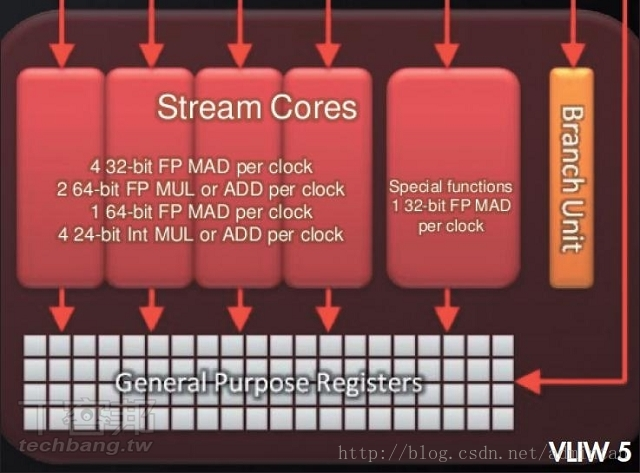
\includegraphics[scale=0.5]{AMD}
					\caption{AMD架构演示}
				\end{figure}			
			
				标注的是Stream Processing Units(统一渲染单元)数量,也可以叫流处理器单元。 
				AMD-ATI从RV670以后,流处理器是\textbf{5个固定的统一渲染单元为一组},4D矢量+1D标量组合。\textbf{其中4个只能进行MADD(乘加)运算,1个可以进行超运算(函数等运算)}。\textit{因为是5个固定为一组,不能拆分,所以遇到纯标量运算时就会有4个SPU处于闲置状态而无法加入其它SP组合协助运算}。但换句话说如果分配得当让每个SPU都充分工作,那么AMD显卡的效率可是非常高的。\textbf{这也是玩家公认A卡驱动提升性能比N卡要高},但也就是这个原因导致A卡驱动设计难度非常高,游戏想要为A卡优化的难度也一样很高。 
				
	\section{更高层-硬件流程}
		\subsection{数据存储转换}
		 	资源信息和指令信息由\textbf{硬盘}经过CPU调度 传输到\textbf{内存}中转,再传输进\textbf{显存}中备用.
		 		\begin{figure}[H]
		 			\centering
		 			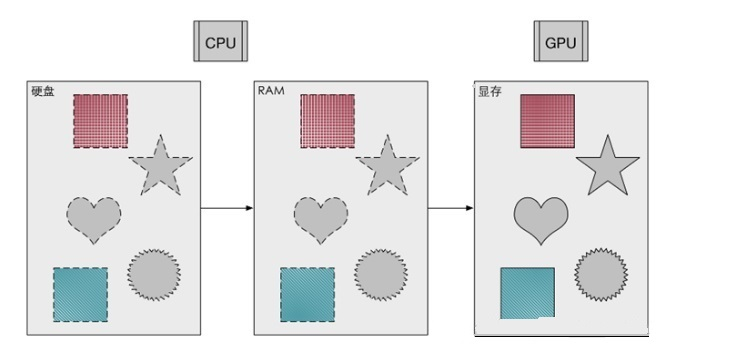
\includegraphics[scale=1]{transfer}
		 			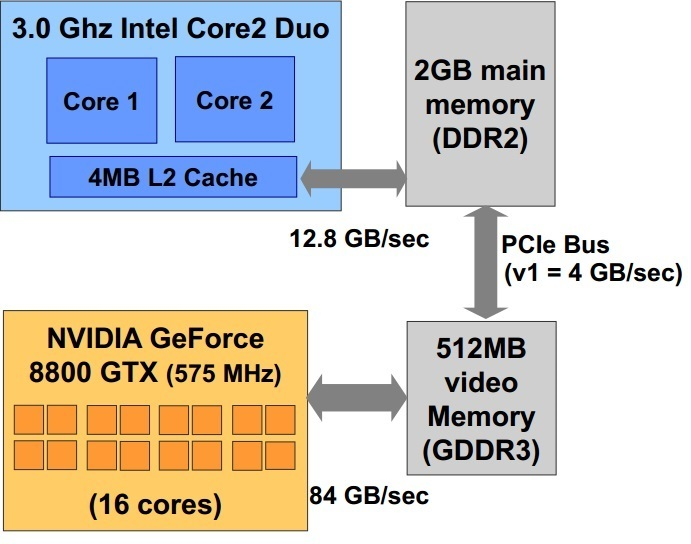
\includegraphics[scale=0.9]{transfer2}
		 			\caption{资源转移}
		 		\end{figure}
		
			由图中的典型的带宽可见 \textbf{GPU和显存之间的内部带宽} 要比单纯的\textbf{系统总线带宽}要高很多。
			所以典型情况下\textbf{渲染资源和渲染指令都被加载进显存}, 所以GPU\textit{在渲染过程中} \textbf{只需向显存调度渲染指令},\underline{避免了和系统总线频繁IO}。
				
		\subsection{进入渲染预备状态}
			\begin{figure}[H]
				\centering
				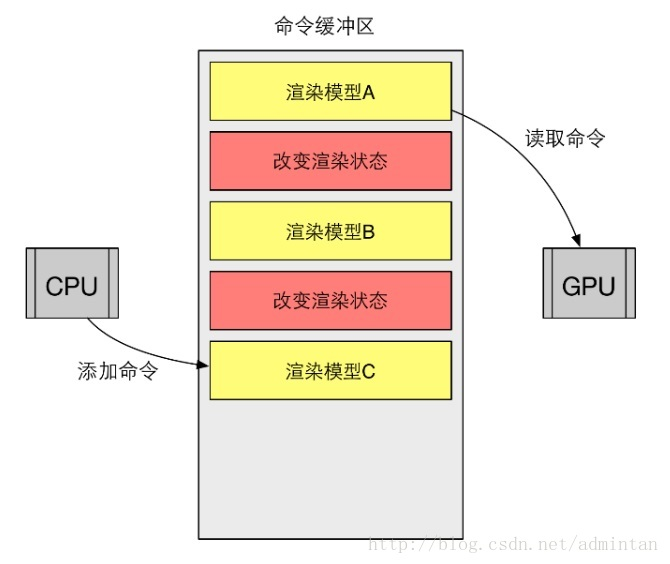
\includegraphics[scale=0.7]{PreShader}
				\caption{渲染预备状态}
			\end{figure}
			
			此时GPU的\textbf{显存越大则依靠CPU的加载额外渲染指令的需要就越少},显存中的信息一般包括: 
			显存和内存一样用于存储GPU处理过后的数据,在显存中有几种不同的储存区域,用于储存不同阶段需要的数据。 
			\begin{enumerate}
				\item \textbf{顶点缓冲区}:用于储存从内存中传递过来的顶点数据。
				\item \textbf{索引缓冲区}:用于储存每个顶点的索引值,我们可以根据索引来使用相应的顶点 
				\item \textbf{纹理缓冲区}:用于储存从内存中传递过来的纹理数据 
				\item \textbf{深度缓冲区}:用于存储每个像素的深度信息
				\item \textbf{模板缓冲区}:用于存储像素的模板值,且模板缓冲区域深度缓冲区公用一片内存。
				\item \textbf{颜色缓冲区}:用于储存像素的颜色数据
			\end{enumerate}	
			
	\section{软件}   
		\begin{figure}[H]
			\centering
			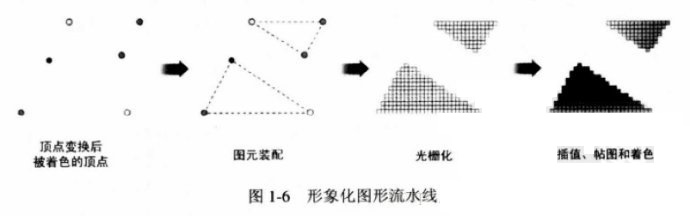
\includegraphics[scale=0.59]{ShaderPro}
			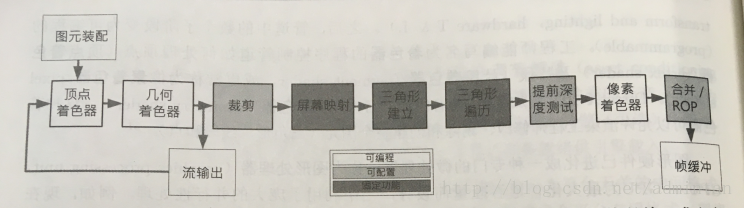
\includegraphics[scale=0.69]{ShaderProc}
			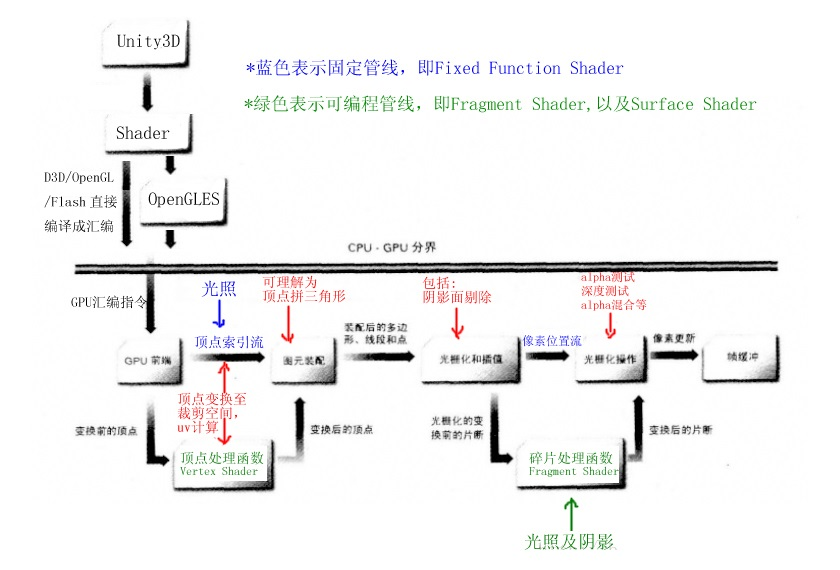
\includegraphics[scale=0.59]{ShaderPro2}
			\caption{Shader 流程(1,4)}
		\end{figure}
	
	
\chapter{书籍推荐}
	
	GPU Gems:\url{https://developer.nvidia.com/gpugems/GPUGems/gpugems_ch01.html}
	
	Real Time Rendering
	
	Uniyt Shader 入门精要
	
\end{document} 
 		    